\documentclass[a4paper]{article}

\usepackage[english]{babel}
\usepackage[utf8]{inputenc}
\usepackage{amsfonts}
\usepackage{amsmath}
\usepackage{amstext}
\usepackage{algorithm,algorithmic}
\usepackage{caption}
\usepackage{pifont}
\usepackage{pdfpages}
\usepackage{setspace}
\usepackage{subcaption}
\usepackage{graphicx}
\usepackage{enumerate}
\usepackage{listings}
\usepackage{float}
\usepackage{enumitem}
\usepackage[colorinlistoftodos]{todonotes}
\usepackage{titlesec}
\usepackage{titling}
\usepackage{fancyhdr}
\pagestyle{fancy}
\DeclareUnicodeCharacter{2212}{-}
\renewcommand\headrulewidth{1pt}
\renewcommand{\labelitemi}{\ding{118}}

\newtheorem{theorem}{Théorème}[section]
\newtheorem{propriete}{Propriété}[theorem]
\newtheorem{corrolaire}{Corrolaire}
\newtheorem{definition}{Définition}
\newtheorem{proof}{Démonstration}


\titleformat*{\section}{\Large\bfseries\sffamily}
\titleformat*{\subsection}{\Large\sffamily}
\titleformat*{\subsubsection}{\large\sffamily}

\title{Mathématiques pour la finance}
\author{Gauthier Marteville}

\lstset { %
    language=Python,
    backgroundcolor=\color{black!5}, % set backgroundcolor
    basicstyle=\ttfamily\small,
    keywordstyle=\color{blue},
    stringstyle=\color{orange},
    commentstyle=\color{green!50!black},
    morecomment=[l][\color{magenta}]{\#},
    numberstyle=\tiny\color{gray},
    emphstyle=\color{purple},
    emph=[1]{vector, cout, cin, endl},
    emphstyle=[1]{\color{purple}},
    emph=[2]{int, double, float, long, char},
    emphstyle=[2]{\color{red}},
    emph=[3]{*},
    emphstyle=[3]{\color{teal}},
    emph=[4]{printf},
    emphstyle=[4]{\color{violet}},
    emph=[5]{define},
    emphstyle=[5]{\color{magenta}},
    tabsize=4,
    showspaces=false,
    showstringspaces=false,
    breaklines=true,
    breakatwhitespace=true,
    escapeinside={(*@}{@*)}
}

\begin{document}

% 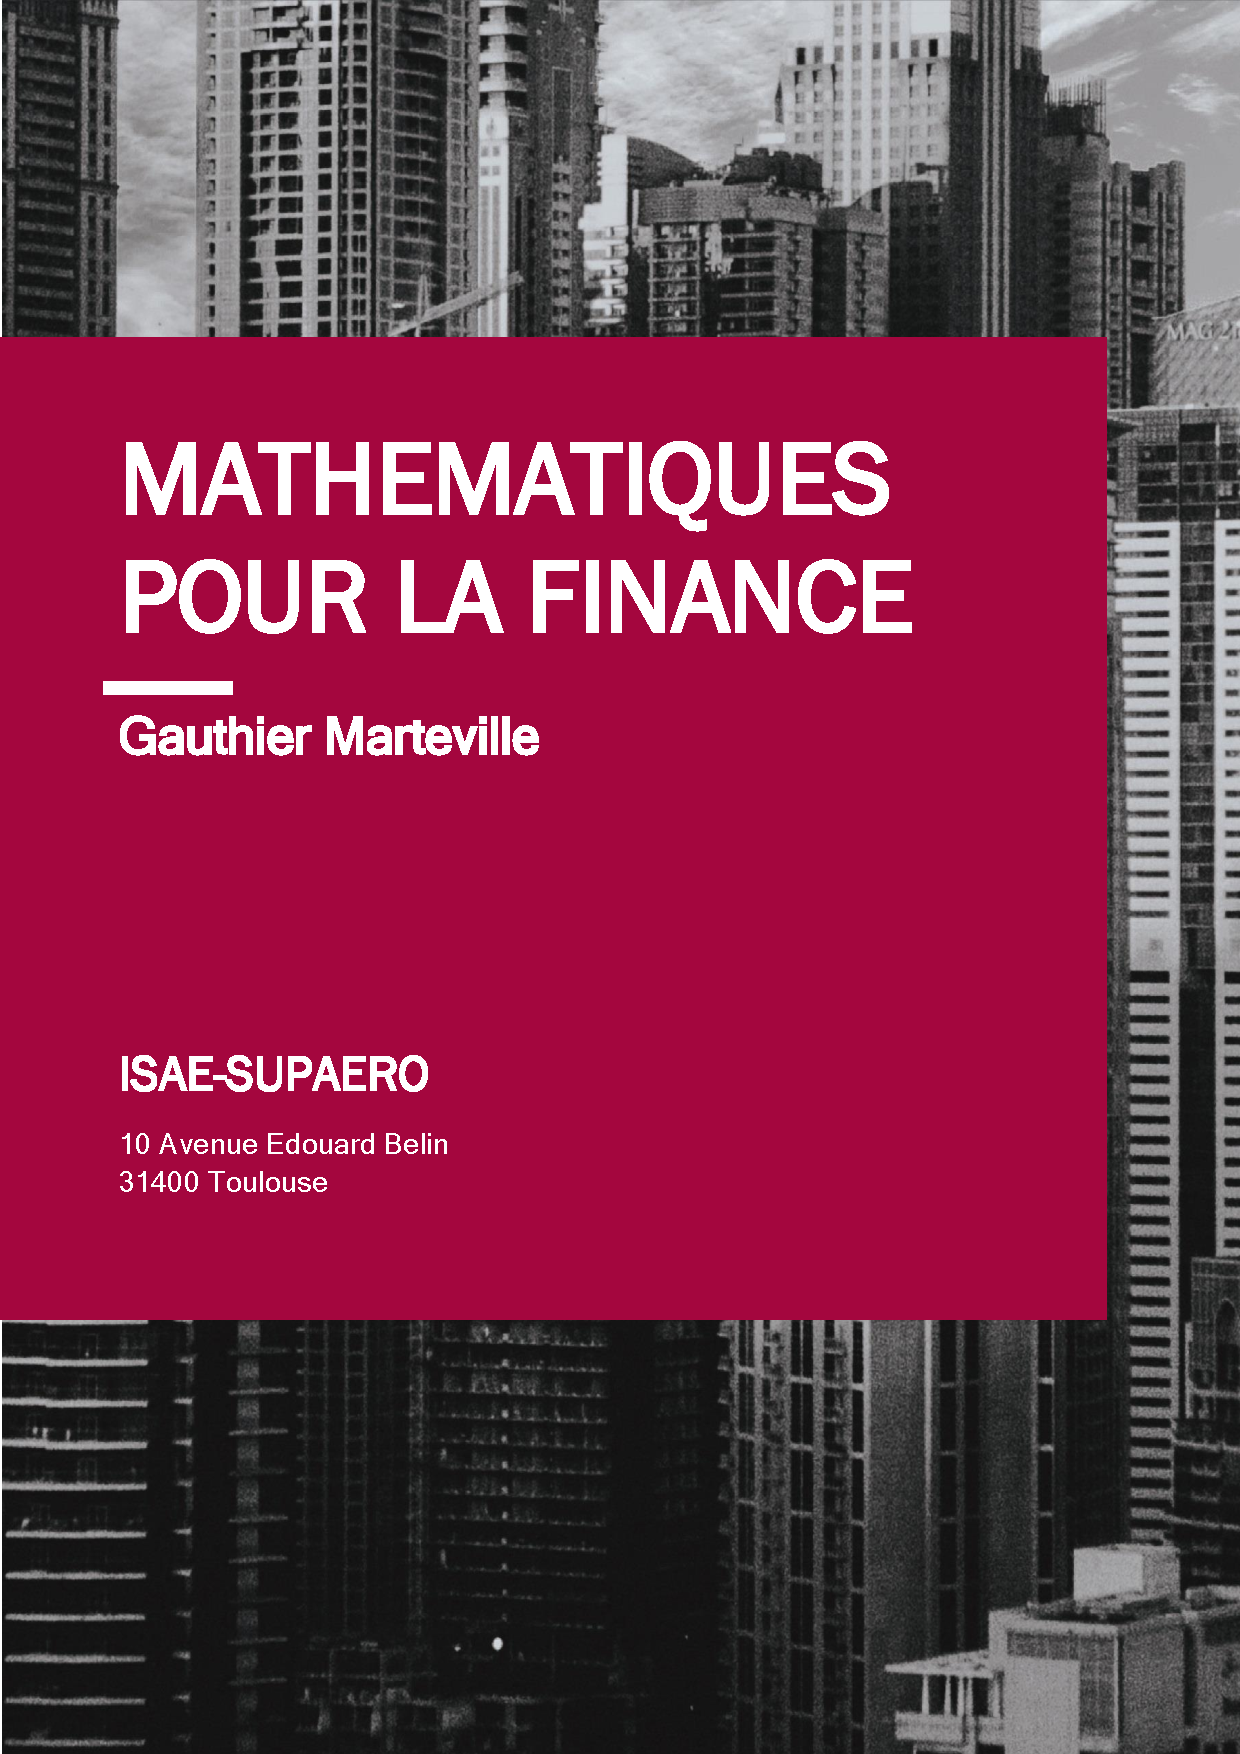
\includepdf{pp.pdf}

\captionsetup[figure]{labelsep= endash,labelfont=sc,justification=justified, font=doublespacing}
\maketitle
\tableofcontents

\section{Propriétés utiles des probabilités}
\subsection{Loi et fonction de répartition}

\subsubsection{Simulation de lois}

\begin{definition}[Fonction quantile]
    Soit $F$ une fonction de répartition. On appelle fonction quantile de $F$ la fonction suivante, définie pour tout $u$ dans $]0;1[$
    \begin{align*}
        F^{-1}(u) = \inf \{x | F(x)\geq u \}       
    \end{align*}
\end{definition}
La fonction quantile peut nous permettre d'établir un lien entre les loi de probabilités, qui est utile lorsque l'on veut simuler une loi.
En effet, lorsqu'une variable aléatoire $X$ est à densité, alors la fonction quantile $F^{-1}$ est l'inverse de la fonction de répartition.

\begin{propriete}
    Soit $U$ une loi uniforme sur un intervalle $I$. Alors la variable aléatoire $X$ définie par $X = F^{-1}(U)$ a pour fonction de répartition $F$.
\end{propriete}
On peut alors par exemple générer une loi exponentielle à partir de la loi uniforme sur $(0,1)$.
Il suffit de prendre pour $F$ la fonction de répartition de la loi exponentielle, $F: x \rightarrow 1 - exp(- \lambda x)$ et de trouver la fonction inverse. Pour un $\lambda > 0$ on a alors 
\begin{align*}
    X = -\frac{1}{\lambda} \log (1-U) =  -\frac{1}{\lambda} \log (U)
\end{align*}
et $X$ suit alors une loi exponentielle, avec $U$ loi uniforme sur $(0,1)$

\subsubsection{Méthodes de rejet}

\subsubsection{Algorithme de Box Muller}
C’est une méthode pour simuler un couple de variables aléatoires indépendantes de loi normale centrée réduite. Elle est basée sur le théorème suivant

\begin{theorem}[Box Muller]
    Soient $R$ et $\Theta$ deux variables aléatoires indépendantes telles que $R^2$ suit une loi exponentielle de paramètre $1/2$ et $\Theta$ suit une loi uniforme sur $[0, 2\pi]$ Alors les variables définies par 
    \begin{align*}
        X = R\cos(\Theta) \text{    et    } Y = R\sin(\Theta)
    \end{align*}
    sont indépendantes et suivent tout deux une loi normale centrée réduite
\end{theorem}
Il suffit donc pour simuler deux variables aléatoires de loi normale centrée réduite de savoir simuler une loi exponentielle et une loi uniforme.
\begin{proof}
    
\end{proof}
\subsection{Espérances conditionnelles}
\label{g}
Etant donné deux variables aléatoires, on peut définir l'espérance de X conditionnée par Y. Elle se note $\mathbb{E}[X|Y]$ et c'est une nouvelle variable aléatoire. Dans le cas où Y est une variable aléatoire discrète, elle est définie comme égale à ${\displaystyle \varphi (Y)}$ où $\varphi$  est la fonction presque partout définie par : ${\displaystyle \varphi (y)=\mathbb{E} [X|\{Y=y\}]}$.
L'espérance de X sachant B, si X est d'espérance finie, est définie par 
\begin{equation}
    \mathbb{E}[X|B]=\sum_{x_i} x_i \mathbb{P}_B (X=x_i)
\end{equation}
Dans le cas général on note $\mathbb{E}[X|Y]$ l'espérance conditionnellement à une variable aléatoire, par le biais de la tribu engendrée par cette variable aléatoire $\mathbb{E}[X|\sigma (Y)]$.\\
\vspace{5mm}\\
\begin{theorem} Soient $X$, $Y$ et $Z$ des variables aléatoires réelles sur un espace de probabilité. Alors \\
\begin{enumerate}[label=\textit{(\roman*)}]
    \item Espérance de l'espérance conditionnelle : $\mathbb{E}\big[\mathbb{E}[X|Y]\big] = \mathbb{E}[X]$
    \item Si Z est $\mathcal{F}$-mesurable, $\mathbb{E}[XZ|\mathcal{F}] = Z\mathbb{E}[X|\mathcal{F}]$
    \item Si X est $\mathcal{F}$-mesurable, $\mathbb{E}[X|\mathcal{F}] = X$
    \item \textit{Inégalité de Jensen}. Si $\phi$ est convexe et si $\phi(X)$ est intégrable alors, Si X est $\mathcal{F}$-mesurable, on a $\mathbb{E}[\phi(X)|\mathcal{F}] \geq \phi\big(\mathbb{E}[X|\mathcal{F}]\big)$
    \item \textcolor{red}{important. (propriété du double conditionnement} Seul reste le conditionnement par \textbf{la tribu la plus petite}: Si $\mathcal{F}_n \subset \mathcal{F}_{n+1}$ alors,
    \begin{center}
        $\mathbb{E}[\mathbb{E}(X|\mathcal{F}_{n+1})|\mathcal{F}_n] = \mathbb{E}[X|\mathcal{F}_n]$
    \end{center}
\end{enumerate}
\end{theorem}
\subsection{Théorème Central Limite}
Ce théorème nous assure la convergence en loi d'une somme de variables aléatoires i.i.d. vers la loi normale centrée réduite. C'est-à-dire que cette somme tend en loi vers une variable aléatoire Gaussienne.\\

\begin{theorem}[Théorème Central Limite]
Soit un entier naturel $N$ et soient $(X_i)_{i\in\mathbb{N}_N}$ des variables aléatoires i.i.d suivant une loi $D$. On suppose qu'il existe pour chaque $X_i$ une espérance finie $\mu$ et un écart-type $\sigma$. On pose $S_n = \sum_{i\in\mathbb{N}_N} X_i$. Alors l'espérance de $S_n$ est $n\mu$ et son écart-type vaut $\sqrt{n}\sigma$. De plus pour $n$ assez grand la loi normale $\mathcal{N}(n\mu, \sqrt{n}\sigma)$ est une bonne approximation de la loi de $S_n$.
Plus formellement, On pose
\begin{equation}
    \overline{X_n} = \frac{S_n}{n} = \frac{\sum_{i=1}^{N}X_i} {n}
\end{equation}
et \begin{equation}
    Z_n = \frac{\overline{X_n} - \mu}{\sqrt{n} \sigma}
\end{equation}
Alors le théorème central limite nous assure que la suite de V.A. $(Z_n)_{n\in\mathbb{N}}$ converge en loi vers $\mathcal{N}(0,1)$\\
\end{theorem}

\begin{proof}[Démonstration]
 
Supposons que $X_1, X_2, ..., X_n$ soient des variables aléatoires indépendantes et identiquement distribuées avec une moyenne $\mu$ et une variance $\sigma^2$. Alors, la somme $S_n = \sum_{i=1}^n X_i$ suit approximativement une distribution normale avec une moyenne $E[S_n] = n\mu$ et une variance $Var[S_n] = n\sigma^2$, lorsque $n$ est grand. En d'autres termes, nous pouvons écrire :

$$\lim_{n\rightarrow\infty} P\left(\frac{S_n - n\mu}{\sigma\sqrt{n}} \leq x\right) = \Phi(x)$$

où $\Phi(x)$ est la fonction de répartition de la distribution normale standard.

Pour démontrer le théorème central limite, commençons par calculer l'espérance et la variance de $S_n$ :
\begin{align*}
E[S_n] &= E\left[\sum_{i=1}^n X_i\right] = \sum_{i=1}^n E[X_i] = \sum_{i=1}^n \mu = n\mu
\end{align*}
De même, nous avons :
\begin{align*}
Var[S_n] &= Var\left[\sum_{i=1}^n X_i\right] = \sum_{i=1}^n Var[X_i] \quad = \sum_{i=1}^n \sigma^2 = n\sigma^2
\end{align*}

Nous pouvons maintenant utiliser la loi des grands nombres pour affirmer que la moyenne empirique $\overline{X} = \dfrac{S_n}{n}$ converge vers la moyenne théorique $\mu$ lorsque $n$ devient grand. En d'autres termes, $\overline{X}$ est un estimateur convergent de $\mu$. Ainsi, nous pouvons écrire :

$$\lim_{n\rightarrow\infty} P\left(\frac{\overline{X} - \mu}{\sigma/\sqrt{n}} \leq x\right) = \Phi(x)$$

où $\Phi(x)$ est la fonction de répartition de la distribution normale standard. En multipliant numérateur et dénominateur par $\sqrt{n}$, nous obtenons :

$$\lim_{n\rightarrow\infty} P\left(\frac{\overline{X} - \mu}{\sigma/\sqrt{n}} \leq x\right) = \lim_{n\rightarrow\infty} P\left(\frac{\overline{X} - \mu}{\frac{\sigma}{\sqrt{n}}} \leq x\sqrt{n}\right) = \Phi(x\sqrt{n})$$

Maintenant, considérons la variable $Z_n = \dfrac{S_n - n\mu}{\sigma\sqrt{n}}$. Nous avons :
\end{proof}


\subsection{Inégalité de Markov}
\begin{theorem}[Inégalité de Markov]
Soit $Z$ une variable aléatoire réelle définie sur un espace probabilisé $(\Omega, \mathcal{A}, \mathbb{P})$ supposée presque surement positive ou nulle. Alors
\begin{equation}
    \forall a > 0, \hspace{2mm} \mathbb{P}(X \geq a) \leq \frac{\mathbb{E}[X]}{a}
\end{equation}
\end{theorem}
\begin{corrolaire}[Inégalité de Markov généralisée] On suppose $\Phi$ une fonction positive croissante sur un intervalle non trivial $I$. Soit $Y$ une variable aléatoire réelle définie sur $(\Omega, \mathcal{A}, \mathbb{P})$ telle que $\mathbb{P}(Y \in I) = 1$. Alors
\begin{equation}
    \forall b \in I, \Phi(b) > 0, \hspace{2mm} \mathbb{P}(Y \geq b) \leq \frac{\mathbb{E}[\Phi(b)]}{\Phi(b)}
\end{equation}
\end{corrolaire}
\begin{theorem}[Inégalité de Bienaymé-Tchebychev] Soit $X$ une variable aléatoire de variance finie $\sigma^2$ et d'espérance $\mu$. Alors pour tout réel strictement positif $\alpha$,
\begin{equation}
    \mathbb{P}(|X - \mu| \geq \alpha) \leq \frac{\sigma^2}{\alpha^2}.
\end{equation}
\end{theorem}
\subsection{Exercices}
\subsubsection{Variable définie par une fonction de répartition}
On considère une loi normale centrèe réduite $\mathcal{N}(0,1)$ et deux réels $a$ et $b$. Montrer que 
\begin{align*}
    \mathbb{E}[\Phi(aX+b)] = \Phi\bigg(\frac{b}{\sqrt{1+a^2}}\bigg)
\end{align*}
Avec $\Phi$ la fonction de répartition de la loi normale centrée réduite.
\vspace{0.5mm}
\textbf{Démonstration.} On peut écrire
\begin{equation*}
    \mathbb{E}[\Phi(aX+b)] =  \mathbb{E}[\mathbb{P}(Y \leq ax+b | X=x)] =  \mathbb{E}[\mathbb{P}(Y-ax \leq b | X=x)]  = \mathbb{P}(Y -aX\leq b)
\end{equation*}
Or $Y-aX \sim\mathcal{N}(0, 1+a^2)$ d'où le résultat.

\section{Chaines de Markov}
\subsection{A propos des graphes}

\begin{enumerate}
  \item \textbf{Probabilité d'Existence d'une Arête :} Dans un graphe aléatoire \( G(n, p) \), la probabilité qu'il existe une arête entre deux sommets donnés est \( p \). Cela signifie que chaque paire de sommets est connectée indépendamment avec une probabilité \( p \).

  \item \textbf{Propriétés Asymptotiques :} Lorsque le nombre de sommets \( n \) devient très grand, certains résultats asymptotiques intéressants émergent. Par exemple, le modèle \( G(n, p) \) peut exhiber des transitions de phase où des propriétés structurelles importantes changent de manière significative.

  \item \textbf{Composantes Connexes :} En fonction de la probabilité \( p \), un graphe aléatoire peut avoir une unique composante connexe géante lorsque \( p \) dépasse un certain seuil critique. En dessous de ce seuil, des petites composantes connexes isolées peuvent apparaître.

  \item \textbf{Degré Moyen :} Le degré moyen d'un sommet dans un graphe aléatoire \( G(n, p) \) est \( (n-1)p \). Cela donne une indication de la densité des connexions dans le graphe.

  \item \textbf{Propriétés de Phase de Transition :} Certains graphes aléatoires passent par des phases de transition, où des propriétés comme la connectivité globale changent brusquement en fonction de la probabilité \( p \).

\end{enumerate}

Les graphes aléatoires sont des outils puissants pour modéliser et analyser des systèmes complexes, et leur étude a des implications importantes dans divers domaines, y compris l'informatique, la physique statistique et les sciences sociales.


\subsection{Processus de Markov}
\begin{definition} Un processus de Markov $(X_n)_{n\geq 0}$à temps discret est un processus stochastique vérifiant la propriété de Markov. \\
\begin{equation}
    P(X_{n+1}|X_n,X_{n-1}, \dots, t_0) = P(X_{n+1}|X_n)
\end{equation}
\end{definition}
\subsection{Hiden Markov Model (HMM)}


\section{Mouvements Browniens}
\subsection{Définition}
\begin{definition}[Mouvement Brownien]
Un mouvement brownien est un processus stochastique $(B_t)_{t\geq 0}$ continu qui modélise le mouvement aléatoire d'une particule dans un fluide. Il vérifie les trois propriétés suivantes
\begin{enumerate}[label=\textit{(\roman*)}]
    \item (Acroissements indépendants) Pour tous $s, t$ tels que $t >s$ l'acroissement $B_t-B_s$ est indépendant du processus $(B_u)_{0\leq u<s}$.
    \item (Accroissements stationnaires et gaussiens) Quels que soient les temps $t$ et $s$ tels que $t > s$, l'accroissement $B_{t} - B_{s}$ est une variable aléatoire normale de moyenne nulle et de variance $t − s$.
    \item $(B_{t})_{t\geq 0}$ est presque sûrement continu, c'est-à-dire pour presque toute réalisation, la fonction $t\mapsto B_{t}(\omega )$ est continue.
\end{enumerate}
Si $X_0=0$ on dit que le mouvement brownien est \textbf{standard}.
\end{definition}
\subsection{Propriétés}
\subsubsection{Inversion temporelle - Stabilité}
\begin{propriete}
    Le processus $(tB_{\frac{1}{t}})$, qui s'annule en $t=0$, est un mouvement brownien. \\
\end{propriete}
\begin{propriete}
    Pour tout $c>0$, le processus $(cB_{\frac{1}{c^2}})$ est un mouvement brownien. On dit qu'il est stable d'indice 2.
\end{propriete}

\subsubsection{Propriété de Markov forte}
\begin{propriete}
     Le mouvement brownien vérifie la propriété de Markov forte. Pour tout temps d'arrêt $T$, conditionnellement à $(T<+\infty)$, le processus $(B_t ^T)_{t\geq 0} = (B_{t+T}-B_T)_{t\geq 0}$ est un mouvement brownien indépendant de $(B_s)_{0\leq s<T}$
\end{propriete}
\subsubsection{Principe de reflection}
\begin{theorem}
    Soit $T$ un temps d'arret et $(B_t)_t$ un Brownien standard. Alors le \textit{Reflected brownian motion at the stopping time $T$} défini par:
    \begin{equation*}
         B_T^* = B_t \textbf{1}\{ t \leq T \} + (2B_T-B_t) \textbf{1} \{ t > T \}
    \end{equation*}
    Est aussi un brownien standard. \\
\end{theorem} 
\begin{proof}
    On utilise la propriété de Markov forte aux deux browniens $(B_{t+T} - B_t)_t$ et $\bigg(-(B_{t+T} - B_t)\bigg)_t$     
\end{proof} 
\vspace{1mm}

\textbf{Application.} On peut ainsi montrer la propriété suivante:
\begin{propriete}
    Pour tout mouvement brownien $(B_s)_s$ on a la relation
    \begin{equation*}
        \mathbb{P}(\max_{0\leq s \leq t} B_s \geq a) = 2 \mathbb{P}(B_t \geq a)
\end{equation*}
\end{propriete}
\begin{proof}
    \begin{figure}
    \centering
    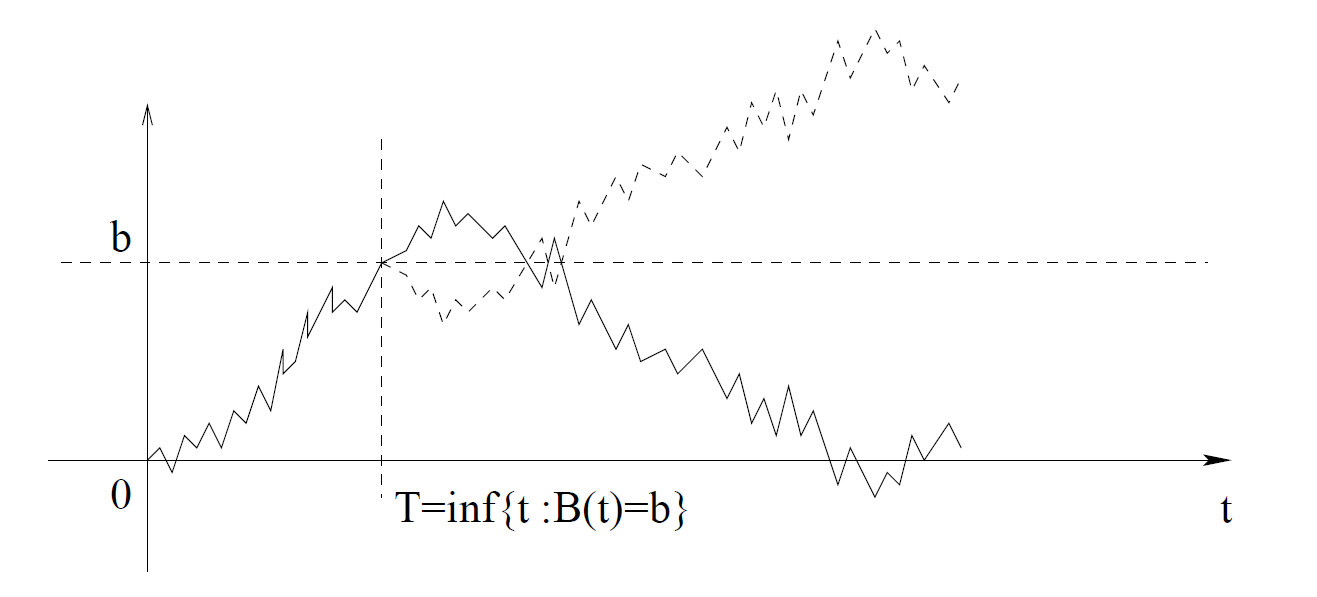
\includegraphics[scale=0.5]{reflection principle.png}
    \caption{Mouvement brownien réflechi du temps d'arret $T$}
    \label{fig:enter-label}
\end{figure}
Posons $M_t = \max_{0\leq s \leq t} B_s$. On peut déja affirmer que $M_t \geq 0$ car $B_0 = 0$ et $(M_t)_t$ est décroissant en $t$.
On pose $T = \inf\{s\geq 0 , B_s=a\}$  et $B_t^*$ le brownien réflechi de $T$. Alors
\begin{equation*}
    \{M_t > a\} = \{ M_t > a \cap ( B_t > a \sqcup B_t \leq a )\} =
    \{ (M_t > a \cap B_t > a) \sqcup (M_t > a \cap B_t \leq a) \}
\end{equation*}
On a donc 
\begin{equation*}
    \mathbb{P}(M_t > a) = \mathbb{P}((M_t > a \cap B_t > a)) + \mathbb{P}((M_t > a \cap B_t \leq a)) = \mathbb{P}(B_t > a) + \mathbb{P}(B_t^* \geq a)
\end{equation*}
Par le principe de réflection, on obtient le résultat.

\end{proof}

\subsubsection{Exercices}
\textbf{Ex.1 -- Deutsche Bank SHL question}
Calculer $\mathbb{P}(B_1 > 0, B_2 >0, \inf_{t \in [1,2]} B_t < 0)$
On utilise le brownien réflechi par le temps d'arret $\tau = \{ \inf t, B_t=0, t>1 \}$ et on remarque que 
\begin{equation*}
\mathbb{P}(B_1 > 0, B_2 >0, \inf_{t \in [1,2]} B_t < 0) = \mathbb{P}(B_1 > 0, B_2 <0)
\end{equation*}
Et on obtient ainsi
\begin{equation*}
    \mathbb{P}(B_1 > 0, B_2 >0, \inf_{t \in [1,2]} B_t < 0) = 1/8
\end{equation*}
\textbf{Ex. 2 -- Fonction de répartition} Soit $B$ un mouvement brownien et $x \in \mathbb{R}_+$. Calculons $\mathbb{P}(|B_t|>x)$.
\\
Si $X \sim \mathcal{N}(0,1)$, On a $\mathbb{P}(|B_t|>x)=\mathbb{P}(|X|>\frac{x}{\sqrt{t}}=2N\bigg( - \frac{x}{\sqrt{t}} \bigg)$

On note $N(x)$ la fonction de répartition de la loi normale. On rappelle que 
\begin{equation}
    N(x) = \int_{-\infty}^{x} \frac{1}{\sigma \sqrt{2\pi}}\exp{-\frac{(x-\mu)^2}{2\sigma^2}}
\end{equation}
On remarque alors que les réalisations $x$ de $B_t$ vérifient $N(x)+N(-x)=1$
\begin{figure}[H]
\centering
    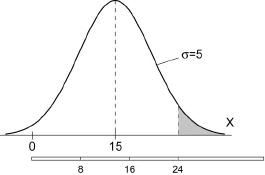
\includegraphics[scale=0.6]{loinormale.png}
    \caption{Fonction de répartition de la loi normale}
    \label{fig:my_label}
\end{figure} 
On a alors
\begin{center}
    $\mathbb{E}[N(B_t)]+\mathbb{E}[N(-B_t)]=1$
\end{center}
Or $B_t$ et $-B_t$ suivent la meme loi. Alors $\mathbb{E}[N(B_t)]=\frac{1}{2}$.

\subsection{Lemme d'Itô}
Le lemme d'Itô permet de résoudre des équations différentielles stochastiques (EDS) très utile pour manipuler le modèle de Black-Scholes (cf. après).
\begin{theorem}[Lemme d'Itô]
Soit $X_t$ un processus stochastique de la forme 
\begin{align*}
    X_t = X_0 + \int_{0}^{t} \mu_s ds + \int_{0}^{t} \sigma_s dB_s
\end{align*}
On peut aussi formuler la version différentielle de l'énoncé i.e. le processus $X_t$ vérifie
\begin{align*}
    dX_t = \mu_t dt + \sigma_t dB_t
\end{align*}
Avec $\sigma_t$ et $\mu_t$ des processus aléatoire et $B_t$ un mouvement brownien. Alors si $f(X_t, t)$ est une fonction de classe $\mathcal{C}^2$ alors on peut écrire
\begin{equation}
    d( f(X_t, t)) = \frac{\partial f}{\partial t}dt + \frac{\partial f}{\partial x}dX_t + \frac{1}{2}\frac{\partial^2 f}{\partial x^2} \sigma_t^2 dt 
\end{equation}
On peut écrire aussi sous la forme, grace à la relation entre $X_t$, $dt$ et $dW_t$
\begin{align*}
     d(f(t,X_t)) = \bigg( \frac{\partial f}{\partial t} + \mu X_t\frac{\partial f}{\partial x} + \frac{1}{2}\frac{\partial^2 f}{\partial x^2} \sigma_t^2 \bigg) dt + \sigma \frac{\partial f}{\partial x} X_t dW_t
\end{align*}
\end{theorem}
Le lemme d'Ito donne une formule pour calculer la dérivée d'une fonction aléatoire en termes des dérivées du processus stochastique sous-jacent.

\subsection{Intégrale d'Itô}
\textbf{Définition.} Pour une fonction $f : [0,T] \rightarrow \mathbb{R}$ (peut etre aléatoire) et $W$ un brownien, l'Intégrale d'Itô est définie par:
\begin{equation}
    \int_{0}^{T} f(t)dW_t = \lim\limits_{N \to \infty} \sum_{n=0}^{N} f(t_n)(W_{n+1}-W_n)
\end{equation}
\begin{propriete}[Isométrie d'Itô]
Pour toute fonction $f,g$ non anticipative de $W$, de moment d'ordre 2 fini, alors
\begin{equation}
    \mathbb{E}\bigg( \int_{0}^{t} f(s)dW_s \bigg)\bigg( \int_{0}^{t} g(s)dW_s \bigg) = \mathbb{E} \int_{0}^{t} f(s)g(s)dt
\end{equation}
\end{propriete}
\textit{Exemple.} On cherche à calculer, pour $W$ un brownien standard, $\mathbb{E} (W_t \int_{0}^{t}s dW_s)$.
On a alors 
\begin{align}
    \mathbb{E} \bigg(W_t \int_{0}^{t} s dW_s \bigg) = \mathbb{E}\bigg( \int_{0}^{t} 1 \dot dW_s \bigg)\bigg( \int_{0}^{t} dW_s \bigg) = \mathbb{E} \int_{0}^{t} 1\dot sds = 
\end{align}

\subsection{Mouvements Browniens multidimensionnels}

\subsubsection{Définition et propriétés}
\begin{definition}
Soit $B_t = (B_t^{(1)}, B_t^{(2)}, \dots, B_t^{(n)})^T$ un processus $n$-dimmensionel. On dit que $B_t$ est un mouvement brownien multidimensionnel si les $(B_t^{(i)})_i$ sont des mouvements browniens indépendants entre eux. 
\end{definition}
\begin{theorem}
    Le processus à $n$-dimensions $B_t$ est un mouvement brownien si et seulement si les processus $B^{(i)}$ et $B^{(i)}B^{(j)} - \delta_{i,j} t$ sont des martingales, où $\delta_{i,j}$ désigne le symbole de Kronecker.
\end{theorem}
\begin{proof}
    WIP...
\end{proof}
\subsubsection{Mouvements browniens corrélés}

\begin{definition}[Mouvements browniens corrélés]
On dit de deux mouvements browniens $B_t^1$ et $B_t^2$ qu'ils sont corrélés de coéfficient de corrélation$\rho$ si $B^1(t) B^2(t) - \rho t$ est une martingale.
\end{definition}
Si on dispose de deux mouvements browniens indépendants $W_t$ et $\tilde{W}_t$  et de $\rho \in [-1,1]$ On peut alors construire un processus $\hat{W}_t$ corrélé comme suit:
\begin{align*}
    \hat{W}(t) = \rho W(t) + \sqrt{1 - \rho^2}\tilde{W}(t)
\end{align*}
A l'inverse, en disposant de deux mouvements corrélés $W_t$ et $\tilde{W}_t$ de coéfficient de corrélation $\rho$, on peut construire un processus $\hat{W}_t$ qui sera un mouvement brownien indépendants des deux premiers:
\begin{align*}
    \hat{W}(t) = \frac{1}{\sqrt{1-\rho^2}}(\tilde{W}(t) - \rho W(t))
\end{align*}

\section{Martingales}
\subsection{Introduction}
\begin{definition}[Martingale]
Une séquence $Y = (Y_n, n\geq 0)$ est une martingale suivant une séquence $X = (X_n, n\geq 0)$ si pour tout $n \geq 0$
\begin{enumerate} [label=\textit{(\roman*)}]
\item $\mathbb{E}[Y_n] < +\infty$
\item $\mathbb{E}[Y_{n+1} | X_0, X_1, \dots] = Y_n$
\end{enumerate}
\end{definition}
\begin{definition}[Filtration]
     Une filtration est une suite croissante (pour l'inclusion) de parties d'un ensemble. On définit alors une martingale suivant une filtration $\mathcal{F}$ sur $(\Omega, \mathcal{F}, \mathbb{P})$ comme une paire $(Y, \mathcal{F})=((Y_n, \mathcal{F}_n), n\geq 0)$ telle que :
\begin{enumerate} [label=\textit{(\roman*)}]
\item $\mathbb{E}[Y_n] < +\infty$
\item $\mathbb{E}[Y_{n+1} | \mathcal{F}_n] = Y_n$
\end{enumerate}
\end{definition}
Soit $Y$ une séquence de variables aléatoires adaptées à une filtration $\mathcal{F}$. En posant $X^+ = \max{(0, X)}$ et $X^- = \min{(0, X)}$ on peut définir les supermartingales et les submartingales comme suit: 
\begin{enumerate}[label=\textit{(\roman*)}]
    \item \textbf{supermartingale} : $\mathbb{E}[Y_n] < +\infty$ et  $\mathbb{E}[Y_{n+1} | \mathcal{F}_n] \geq Y_n$
    \item \textbf{submartingale} : $\mathbb{E}[Y_n] < +\infty$ et  $\mathbb{E}[Y_{n+1}| \mathcal{F}_n] \leq Y_n$
\end{enumerate}
\begin{theorem}[Inégalité maximale de Doob] Soit $(M_n)_{n\geq 0}$ une sous-martingale positive. Pour tout $a > 0$ et tout $n\in \mathbb{N}$, on a 
\begin{equation}
    \mathbb{P}\bigg(\underset{0 \leq k \leq n}{\max}M_k \geq a\bigg) \leq \frac{\mathbb{E}[M_n]}{a}
\end{equation}
\end{theorem}
\begin{theorem}[Décomposition de Doob] Une submartingale $(Y, \mathcal{F})$ avec une espérance finie peut être décomposée de la forme suivante:
\begin{equation}
    Y_n = M_n + S_n
\end{equation}
Où $(M, \mathcal{F})$ est une martingale et $(S, \mathcal{F})$ est un processus croissant prédictible.
\end{theorem}
\subsection{Martingales et mouvements browniens}

\textbf{Proposistion 1. $(B_t)_t$ est une martingale} 

\textit{dem.} Les moments d'ordre 1 et 2 sont finis car $B \sim \mathcal{N}(0, t)$. Ensuite, 
\begin{align}
    \mathbb{E}[B_t|F_t] = \mathbb{E}[B_s + (B_t-B_s)|F_s] = B_s + \mathbb{E}[B_t-B_s|F_s] = B_s
\end{align}
car $B_t-B_s$ est indépendant de $\mathcal{F}_n$ (suite croissante de tribus).
\\
\vspace{0.5mm}
\\
\textbf{Proposition 2. $cov(B_s, B_t) = \inf(s,t)$}
\\
\textit{dem.} De la meme manière, $cov(B_t, B_s) = cov(B_s, B_s + (B_t-B_s)) = var(B_s) + cov(B_s-B_0, B_t-B_s) = var(B_s) = s$ si $s<t$ et on a le résultat avec $s>t$.
\\
\vspace{0.5mm}
\\
\textbf{Proposition 3. ${B_t}^2 -t$ est une martingale.}
\\
\textit{dem.} Meme principe que pour les points précédents.
\\
\vspace{0.5mm}
\\
\textbf{Proposition 4. $\exp\bigg( \lambda B_t - \frac{\lambda ^2 t}{2} \bigg)$ est une martingale.}
\\
\textit{dem.} On utilise le fait que si $X \sim \mathcal{N}(\mu, \sigma ^2)$ alors
\begin{equation}
    \mathbb{E}[e^{aX}] = e^{a\mu + \frac{a^2\sigma^2}{2}}
\end{equation}
\subsection{Différence de martingales}
\begin{theorem}[Inégalité de Hoeffding] Soit $(Y, \mathcal{F})$ une martingale. On suppose qu'il existe une suite de réels $(K_i)_{i\in \mathbb{N}}$ telle que pour tout $n$, on ai $\mathbb{P}(|Y_n - Y_{n-1}| \geq K_n) =1$. Alors
\begin{equation}
    \mathbb{P}(|Y_n - Y_0| \geq x) \leq 2\exp{\bigg(-\frac{1}{2}x^2\bigg/ \sum_{i=1}^{n} K_i ^2\bigg)}
\end{equation}
C'est-à-dire que si la martingale est presque sûrement majorée. Il y a une faible probabilité de déviation de $Y_n$ de sa valeur initiale $Y_0$.
\end{theorem}
\subsection{Convergence des martingales}
\begin{theorem}[Convergence des martingales] Soit une submartingale $(Y, \mathcal{F})$. On suppose que $\mathbb{E}[Y_n^+] \leq M$ pour un certain $M$ et pour tout $n$. Alors il existe une variable $Y_{\infty}$ tel que $Y_n \longrightarrow Y_{\infty}$ presque sûrement. De plus,
\begin{enumerate}
    \item \[ Y_{\infty} \] est d'espérance finie si \[ \mathbb{E}|Y_0|< + \infty \]
    \item \[ Y_n \longrightarrow Y_{\infty}\] si la séquence $(Y_n, n \geq 0)$ est uniformément intégrable.
\end{enumerate}
\end{theorem}
\subsection{Stopping Times}
\subsubsection{Motivations} Le principe des \textit{stopping times} repose sur le fait qu'à chaque instant, on a l'information qu'on peut ou non prendre une décision. C'est-à-dire que si on considère un espace probabilisé $(\Omega, \mathcal{F}, \mathbb{P})$ et une filtration $\mathcal{F} = (\mathcal{F}_1, \mathcal{F}_2, \dots)$, on attribue à $\mathcal{F}_n$ l'information disponible à l'instant $n$. Plus précisément, la plus petite $\sigma$-algèbre (au sens de l'inclusion) contenant l'information disponible jusqu'au temps $n$. Les valeurs prises par cette variable aléatoire sont considérées comme des moments d'intérêt.
\subsubsection{Définitions}
\begin{definition}
Un temps d'arrêt $T$ est une variable aléatoire définie par rapport à une filtration $(\mathcal{F}_n)_{n\in \mathcal{N}}$ si,
\end{definition}
\begin{equation}
    \forall n, \hspace{2mm}\{T=n\} \in \mathcal{F} \hspace{1mm} \text{ou encore} \hspace{1mm}\{T\leq n\} \in \mathcal{F}
\end{equation}
\subsubsection{Martingales locale}
\begin{definition}
Un processus stochastique $X_t$ est une \textbf{martingale locale} si il existe une suite de temps d'arrets $(\tau_n)$ telle que $\mathbb{P}(\lim \tau_n = \infty)=1$ and $X_{t\wedge\tau_n}$ est une martingale pour tout $n$.
\end{definition}

\subsection{Théorème de Girsanov}
le théorème de Girsanov indique comment un processus stochastique change si l'on change de mesure.\\ Il donne la manière de passer de la probabilité historique qui décrit la probabilité qu'un \textbf{actif sous-jacent} (comme le prix d'une action ou un taux d'intérêt) prenne dans le futur une valeur donnée à la probabilité risque neutre qui est un outil très utile pour évaluer la valeur d'un dérivé du sous-jacent. \\ 
\vspace{2mm} \\
Soit $X_{t}$ une martingale locale continue par rapport à une filtration $(\mathcal{F}_t)_{t \geq 0}$ satisfaisant les conditions usuelles. On définit l'exponentielle stochastique $Z_t$
\begin{equation}
    Z_t = \exp{\bigg( \int_{0}^{t} \theta_s dW_s - \frac{1}{2} \int_{0}^{t} \theta^2_s ds \bigg)}
\end{equation}
On a montré que si $\theta$ était déterministe constant alors le processus $Z_t$ est alors une martingale. On peut définir une mesure $\mathbb{Q}$ équivalente à la restriction de la mesure $\mathbb{P}$ à $\mathcal{F}_{t}$ à partir de sa densité de Radon-Nikodym. 
\begin{equation}
    d \mathbb{Q} = Z_t d \mathbb{P}
\end{equation}
\begin{theorem}[Théorème de Girsanov]
Si on a les conditions suivantes
\begin{itemize}
    \item $Z_t$ est une vraie martingale, la famille $Q_{t}$ est induite par une mesure $Q$ définie sur toute la tribu $\mathcal{F}_t$ : $Q_{|\mathcal{F}_t} = Q_t$.
    \item $W$ est un brownien sous $\mathbb{P}$
\end{itemize}
alors le processus 
\begin{equation}
    \Tilde{W_t} = W_t - \int_{0}^{t} \theta_s ds
\end{equation}
est un brownien sous $\mathbb{Q}$. 
 \\

\end{theorem}
\vspace{2mm} 
Ce théorème peut être utilisé pour trouver l'unique probabilité risque neutre dans le modèle de Black-Scholes. Ainsi, si un actif suit le processus de diffusion vérifiant : 
\begin{equation}
    \frac{dS}{S} = \mu dt + \sigma dW_t
\end{equation}
Où $W_t$ est un $P$-mouvement Brownien, en effectuant le changement de probabilité suivant : 
\begin{equation}
    \frac{dQ_t}{dP}_{|\mathcal{F}_t} = \exp{ \bigg(  \int_{0}^{t} \frac{r-\mu}{\sigma}dW_s -\frac{1}{2}\bigg( \frac{r-\mu}{\sigma}\bigg)^2 ds\bigg)}
\end{equation}
Le note $\theta = \frac{r-\mu}{\sigma}$, c'est le \textbf{market price of asset risk}.
On obtient une diffusion vérifiant :
\begin{equation}
    \frac{dS}{S} = r dt + \sigma d \Tilde{W_t}
\end{equation}
Où $\Tilde{W_t}$ est un Q-mouvement brownien. Si on note $\tilde{S}$ la valeur actualisée de $S$, on a :
\begin{equation}
    \frac{d\Tilde{S}}{S} = \sigma d \Tilde{W_t}
\end{equation}
Sous la probabilité Q la valeur de notre actif réactualisée est une martingale.
\begin{figure}[H]
\centering
    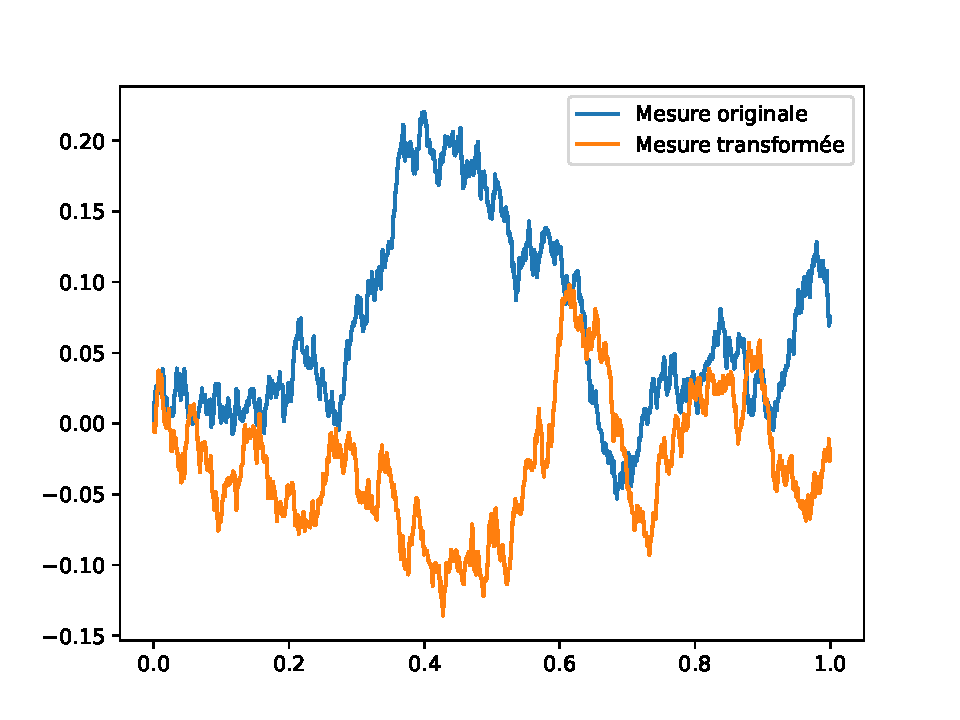
\includegraphics[scale=0.6]{girsqnov.pdf}
    \caption{Processus stochastiques sous la mesure transformée de Girasnov}
    \label{fig:my_label}
\end{figure} 
Le premier processus X est généré selon la mesure de probabilité originale, en utilisant la méthode d'Euler pour simuler l'évolution du processus.
Le deuxième processus Y est généré en utilisant le théorème de Girsanov, en ajoutant un drift proportionnel à la différence entre la mesure transformée et la mesure originale.
Enfin, les deux processus sont affichés sur un graphique, avec la fonction plot de matplotlib. Le graphique montre la différence entre les deux processus, qui est plus grande aux endroits où la mesure transformée est différente de la mesure originale. 

\subsection{Formule de Feynman--Kac}
Cette formule relie la solution d'une équation aux dérivées partielles à une espérance conditionnelle impliquant un processus stochastique. 
\begin{theorem}[Formule de Feynman--Kac]
Soit $f$ une fonction réelle bornée, $\Psi$ une fonction de classe $\mathcal{C}^2$ à support compact $K$ dans $\mathbb{R}$ et $q$ une fonction réelle bornée. Avec $X_t$ vérifiant
\begin{align*}
    dX_t = \mu(X_t,t) dt + \sigma(X_t, t) dW_t
\end{align*}
Alors pour $0 \leq t \leq T$, la formule de Feynman--Kac est
\begin{equation}
    v(t,x) = \mathbb{E} \bigg[ \int_{t}^{T} f(X_s)e^{-\int_{t}^{s} q(X_u)du} ds + e^{-\int_{t}^{T} q(X_s)ds} \Psi(X_T) | X_t=x \bigg]
\end{equation}
et $v$ est solution bornée unique de la SDE avec la condition $v(T,x)=\Psi(x)$
\begin{equation}
    \frac{\partial v}{\partial t} + \frac{\sigma^2(x)}{2} \frac{\partial^2 v}{\partial x^2} + \mu(x) \frac{\partial v}{\partial x} -q(x)v(t,x) + f(t,x) =0
\end{equation}
\end{theorem}

\subsection{Quelques utilisations des martingales}
\subsubsection{Ruine d'un joueur}



\section{Processus de Lévy}

\subsection{Définition}
Un processus stochastique $(X_t)_{t\geq 0}$ est dit \textit{de Lévy} si il vérifie les conditions suivantes:
\begin{enumerate}[label=\textit{(\roman*)}]
\item $X_0 = 0$ ps.
\item (Acroissement indépendants) Pour tout $s < t$, l'acroissement $X_t - X_s$ est indépendant du processus $(X_u)_{0\leq u \leq s}$.
\item (Acroissement stationnaires) Pour tout $s < t$, l'acroissement $X_t - X_s$ est égal en loi au processus  $(X_{t-s})$.
\item $t \mapsto X_t$ est continue ps et limitée à gauche
\end{enumerate}
\textbf{Remarque.} On dit que $t \mapsto X_t$ est limitée à gauche lorsque si le processus $X_t$ est discontinu en un certain $t_0$ alors sa valeur augmente instantanément mais ne peut pas diminuer. \\
\vspace{1mm}
\\
Ils sont utilisés pour modéliser les variations des prix d'actifs financiers, comme les actions et les devises. Les sauts dans les prix, comme les krachs boursiers, peuvent être bien capturés par ces processus.
\subsection{Exemple : les processus de Poisson}


\section{Notions de finance}
\subsection{Les securities}
les titres financiers ou \textit{securities} font référence à des instruments financiers négociables qui représentent une forme de propriété ou de créance. Les securities sont utilisées pour lever des fonds et pour investir dans des entreprises ou des gouvernements.
\subsubsection{Les obligations (\textit{bonds})}
\texttt{https://www.forbes.com/advisor/investing/what-is-a-bond/}
 \begin{enumerate}
        \item \textbf{Corporate bonds.} Investors who purchase corporate bonds become creditors of the company and receive periodic interest payments (coupon) and the return of the principal amount at the bond's maturity date.
        \item \textbf{Treasury bonds.} Government bonds, often referred to as treasuries, are issued by governments to finance their operations. \textcolor{blue}{They are generally considered low-risk investments.}
        \item \textbf{Municipal bonds.} are issued by state and local governments or agencies to fund public projects such as infrastructure improvements or schools. \textcolor{blue}{They often offer tax advantages for investors.}
\end{enumerate}
On définit pour les obligations plusieurs quantités.
\begin{enumerate}
    \item \textbf{Maturity.} La maturité désigne la date à laquelle l'obligation va expirer. i.e. la date à laquelle le \textit{bond issuer} doit retourner l'argent au \textit{bond investor}.
    \item \textbf{Face Value, Par Value.} La valeur nominale est la valeur qui devra etre rembourser à maturité. Généralement, on a $FV = \$ 1000$.
    \item \textbf{Coupon.} Le coupon est le \textit{rate of interest} que le bond issuer va payer à l'investisseur. Par exemple, un bond qui a 3\% de coupon sur un $FV$ de \$1000, le issuer va payer $3\%$ of $\$ 1000 = \$30$ par an jusqu'à maturité.
    Lorsque le coupon est fixe on parle de \textcolor{blue}{Fixed Income (FI)} et lorsqu'il est variable on parle de \textcolor{blue}{Floating Rate Note (FRN)} ou encore \textit{floater}
    \item \textbf{Yield, rate of return.} le rendement d'un bond est variable, contrairement au $FV$,
    \item \textbf{Price.} La plupart des bonds sont tradés après leur emission, on considère deux prices pour les bons, \textit{bid} et \textit{ask}, le premier pour \textbf{le prix maximal que peut mettre un buyer}, le second pour \textbf{le prix minimal que le seller peut céder} le bond.
    \item \textbf{Duration.} La duration d'une obligation est la durée de vie moyenne de ses flux financiers pondérée par leur valeur actualisée. \textcolor{blue}{Plus la duration est élevée, plus le risque est grand.} Elle est fonction de toutes les autres quantités citées plus haut.
\end{enumerate}

\subsubsection{Les actions (\textit{equity, stock})}

Investment growth potential, \textbf{dividends :} many companies pay dividends to investors corresponding to a portion of their profits distributed to shareholders. \textbf{Diversification :}  By investing in stocks of different companies operating in various sectors, you reduce concentration risk. \textbf{Liquidity :}  Stocks are typically liquid, meaning you can buy or sell them relatively easily on stock markets. This liquidity provides flexibility to adjust your portfolio based on market conditions.\\
In summary, equities are one of the primary asset classes in financial markets, representing partial ownership in a company. They offer investment opportunities for those looking to participate in potential company growth and dividend income while being aware of the risks associated with market volatility. Investors should diversify their portfolios and have a long-term investment strategy to make the most of stocks.
\subsection{Les produits dérivés}
Un produit dérivé est un contrat financier dont la valeur dépend de l'évolution d'un actif sous-jacent tel qu'une \textit{action}, une devise, une matière première, un indice boursier, une \textit{obligation} ou un \textit{taux d'intérêt}. Les produits dérivés permettent aux investisseurs de spéculer sur l'évolution future des prix ou des taux, d'assurer leurs positions existantes contre les risques de fluctuations des marchés, ou encore de se protéger contre les pertes potentielles.
\vspace{2mm}
\\ Il existe différents types de produits dérivés, \textbf{notamment les contrats à terme, les options, les swaps et les contrats d'échange}.
\begin{itemize}
    \item Les \textbf{contrats à terme} sont des accords d'achat ou de vente d'un actif à une date future à un prix déterminé à l'avance.
    \item Les \textbf{options} offrent à l'acheteur le droit, mais pas l'obligation, d'acheter ou de vendre un actif sous-jacent à un prix déterminé à l'avance, à une date donnée ou avant celle-ci.
    \item Les \textbf{swaps} sont des contrats d'échange d'actifs ou de flux de trésorerie entre deux parties.
    \item Les \textbf{contrats d'échange} permettent également aux parties d'échanger des flux de trésorerie en fonction de différents taux d'intérêt.
\end{itemize}  
\vspace{2mm}
Les produits dérivés peuvent être utilisés pour diverses finalités, notamment pour couvrir les risques de marché, pour générer des rendements, pour se protéger contre l'inflation ou pour se positionner sur des tendances de marché spécifiques. Toutefois, ils sont également associés à des risques de pertes potentiellement importantes et nécessitent une connaissance approfondie des marchés financiers et des instruments financiers pour être utilisés de manière efficace.
\subsubsection{Les options}
Les options sont des produits financiers dérivés donnant le droit (et non l'obligation) d'acheter (on dit alors \textbf{call}) ou de vendre (on dit alors \textbf{put}) une quantité d'actifs sous-jaçents pendant une période et à un prix connu à l'avance. On paye une prime (prix d'exercice de l'option) pour acquérir ce droit. \\
On distingue les options européennes (on peut exercer son droit uniquement à la fin du contrat) des options américaines (on peut exercer sont droit pendant toute la durée du contrat).
\vspace{2mm} 
\textbf{Variation du prix de l'option.} La prime varie en fonction du sous-jaçent (acxtion, indice, matière prmière, devise, etc) mais également en fonction de l'offre et la demande. Il est donc composé de deux termes, la valeur \textit{intrinsèque} et la valeur \textit{temporelle}. (Source AMF)
\subsubsection{Les futures}
Le future (contrat à terme en français) est un contrat par lequel deux parties s’engagent à acheter (ou vendre) \textbf{une quantité déterminée d’un actif sous-jacent} (une action ou un indice boursier par exemple), à une date d’échéance et à un prix convenus à l’avance. Il permet d’anticiper les variations futures d’un actif sous-jacent et peut donc servir à couvrir un portefeuille contre les fluctuations à venir du marché. Il permet aussi de dynamiser les performances de son portefeuille. Le future constitue un engagement ferme, il doit être exécuté à sa date d’échéance par ses contreparties : l’acheteur du future doit acheter l’actif sous-jacent au prix convenu et le vendeur doit livrer l’actif.
\vspace{2mm} \\
\textbf{Fonctionnement.} Au moment de l’achat (On anticipe une hausse de l’actif sous-jacent) ou de la vente (On anticipe la baisse de l’actif sous-jacent) de future, un dépôt de garantie est requis. C’est une caution qui permet d’assurer la bonne fin des opérations en cas de défaillance d’une ou des parties. Puis, chaque jour, après la clôture du marché, vous recevez des notifications d’appels de marge. Ils correspondent aux profits ou pertes de votre position et dépendent de la réalisation (ou non) de votre anticipation. Ainsi, en cas de bonne anticipation, vous êtes bénéficiaire de l’appel de marge. Dans le cas contraire, vous êtes redevable de l’appel de marge. Dans l’hypothèse où le solde de votre compte ne suffit pas pour faire face à l’appel de marge, votre position peut être soldée et le dépôt de garantie servir à apurer l’appel de marge.

\subsubsection{Les forwards}

Un contrat forward est un contrat à terme \textbf{de gré à gré (Over The Counter -- OTC)}, c’est-à-dire un accord entre un acheteur et un vendeur pour négocier un actif, \textit{habituellement une devise}, à un prix et une date fixés d’un commun accord. Contrairement aux contrats futures, les contrats à terme sont des accords privés entre l’acheteur et le vendeur et, à ce titre, \textbf{ils ne sont pas négociés sur les marchés centralisés}, mais plutôt considérés comme faisant partie du marché OTC. Cela rend les contrats forward plus risqués que les contrats futures. Les principaux facteurs qui déterminent le prix d’un contrat forward sont la valeur marchande de l’actif et le moment où le contrat prendra fin, ce qui est influencé par les taux swap.

\subsubsection{Les swaps}
Un swap est un échange entre deux parties, une sortie de crédit croisé consenti pour une période fixée dès le départ, de quelques jours à quelques mois ou années. Cet échange permet aux contreparties d'échanger une série de flux futurs. Outre la nature du flux échangé, le contrat swap doit spécifier plusieurs éléments : montant nominal, date de départ du contrat, durée, valeur du taux fixe, base de calcul et échéancier des versements, référence du taux variable et échéancier des versements, etc.
\vspace{2mm} \\
\textbf{Fonctionnement.} Les swaps ont pour vocation initiale de réduire l’exposition au risque d’une entreprise ou d’un individu. Aucune transaction n’est effectuée sur le capital : ce sont uniquement les flux d’intérêts qui sont échangés (swapés). \\
Dans le cadre d’une opération de couverture, ils permettent souvent d’échanger un produit financier volatil contre un produit financier plus stable. Dans le cas d’un swap de taux, un taux variable pourra par exemple être échangé contre un taux fixe.
\vspace{2mm} \\
\textbf{Principaux types de swap:} On recense de multiples formes de swap. Parmi les plus fréquents :
\begin{itemize}
    \item Les \textbf{swaps de taux} font figure de poids lourds du marché. Ils sont notamment utilisés par des entreprises endettées à taux fixe qui estiment que les taux vont baisser. Elle trouvent donc intérêt à échanger un taux fixe contre un taux variable pour profiter de cette baisse et inversement (pour la contrepartie).
    \item Les \textbf{Credit Default Swaps (CDS)} procurent une assurance contre un possible défaut, en contrepartie du versement périodique d’intérêt (une sorte d’assurance) jusqu’au terme de l’échange.
    \item Les \textbf{swaps de matières premières} permettent de troquer un prix fixe (par exemple celui du soja) contre un prix variable, le plus souvent calculé comme la moyenne d'un indice sur une période future. 
    \item Les \textbf{swaps de devises} permettent d’échanger les intérêts et la valeur d’un sous-jacent dans une devise contre sa valeur dans une autre devise. 
\end{itemize}

\subsubsection{Tableau récapitulatif}
On peut résumer 


\begin{figure}[h!]
\centerline{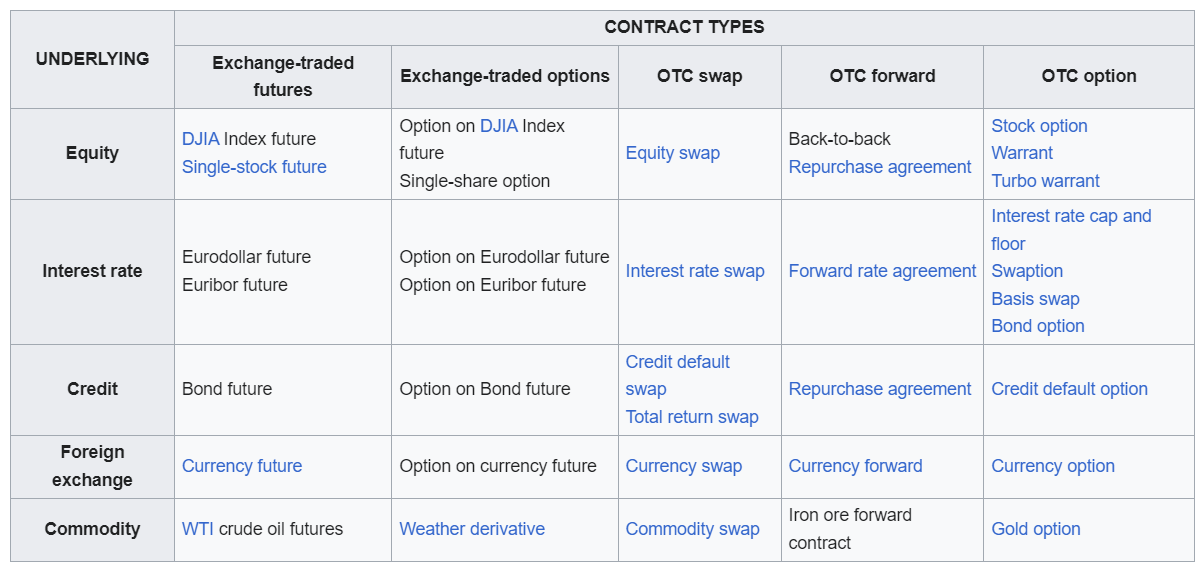
\includegraphics[scale=0.6]{tableau derivaives.png}}
\caption{derivatives}
\end{figure}

\subsection{Les indices}

\subsubsection{VIX volatility index}

Le VIX est un indicateur de volatilité établi tous les jours par le Chicago Board Options Exchange (CBOE). Il est calculé en prenant la moyenne des volatilités \textbf{annuelles} sur les calls et puts sur indice S\&P500. On a introduit aussi un indice de \textit{vol de vol} VVIX qui mesure la volatilité du VIX.

\begin{figure}[H]
    \centering
    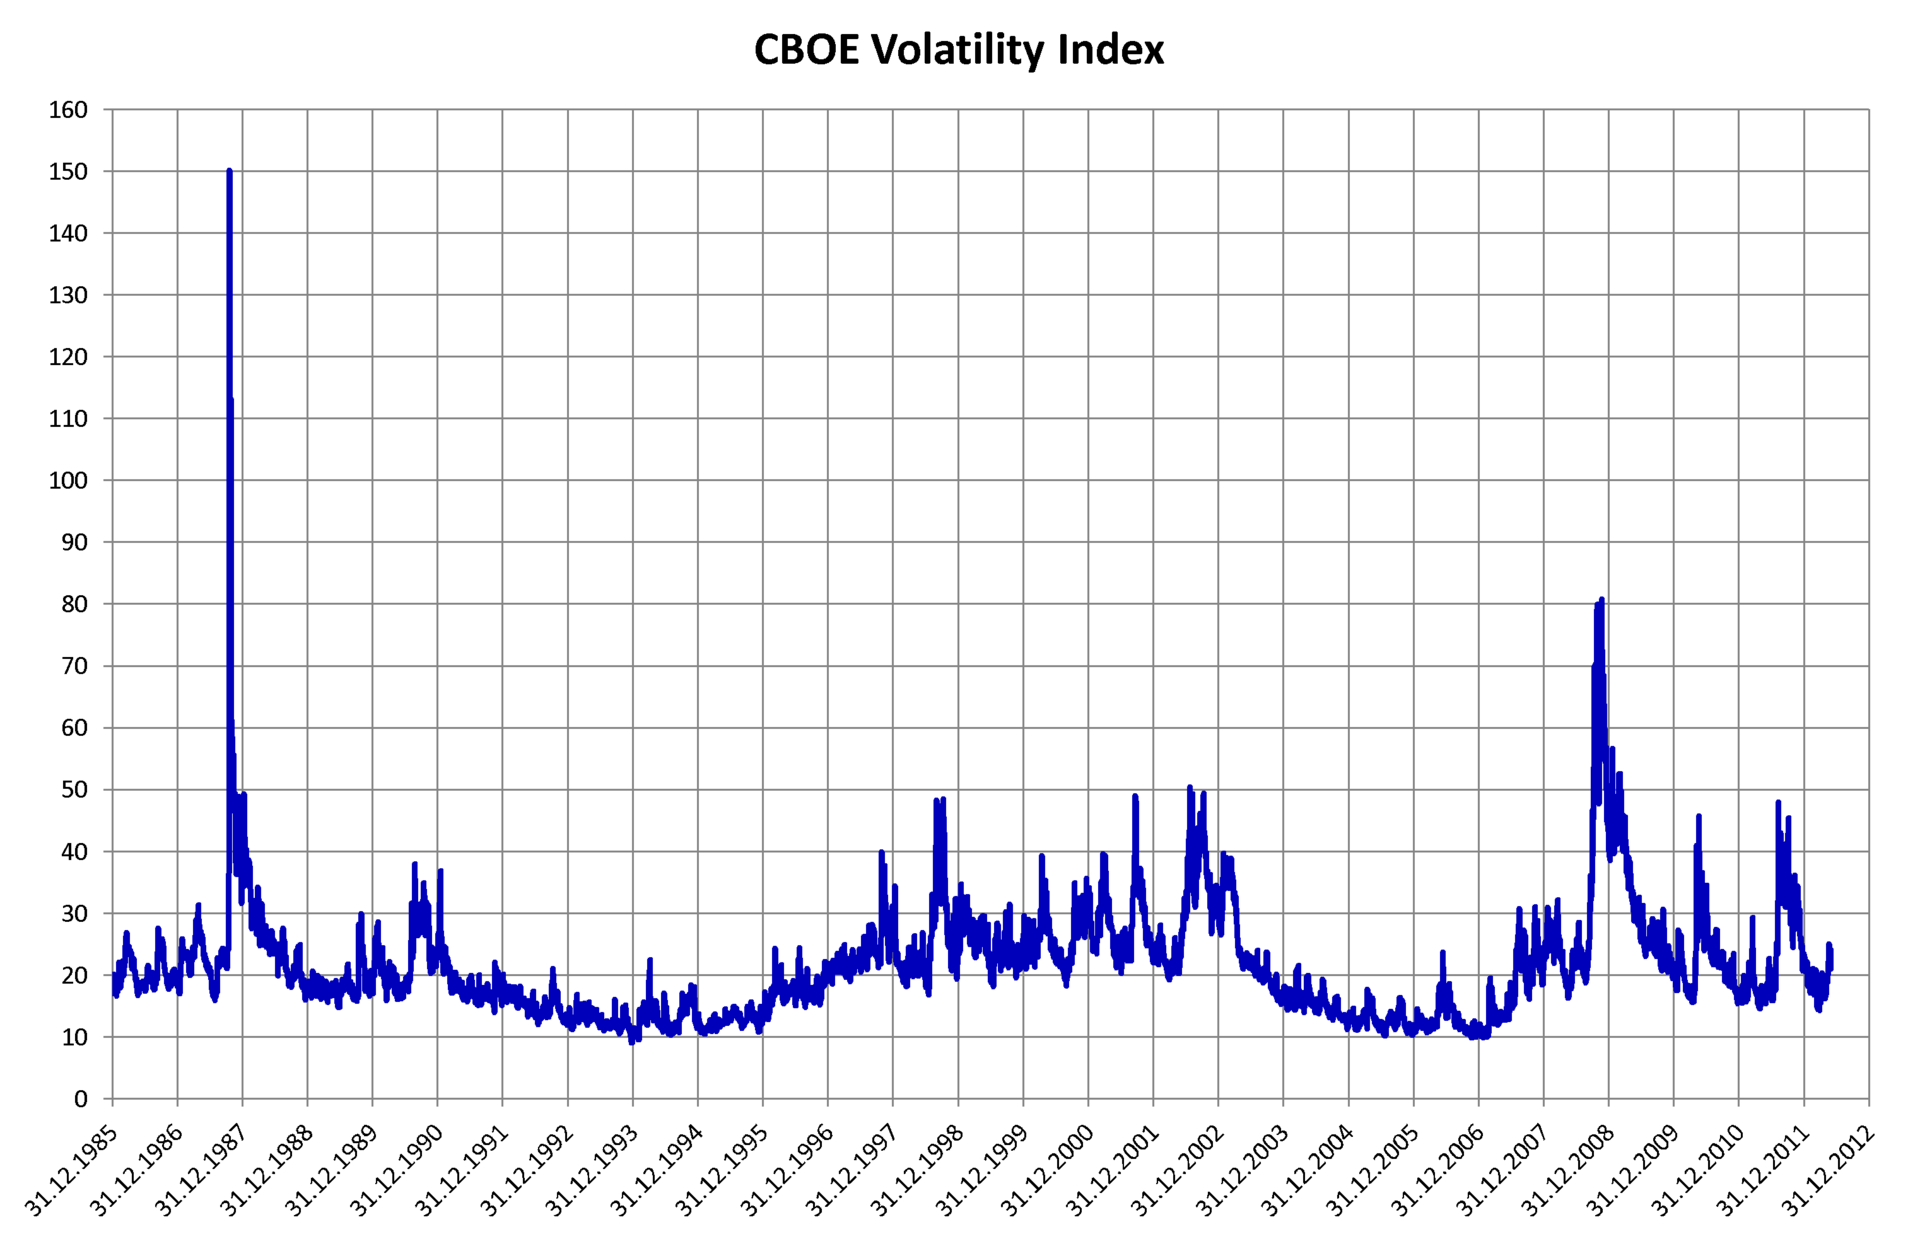
\includegraphics[scale=0.15]{vix.png}
    \caption{Evolution du VIX de 1985 a 2012 (Wikipedia)}
    \label{fig:enter-label}
\end{figure}

Des indices de vol sur d'autres indices existent aussi tels que le VXN (indice de vol sur NASDAQ), le VXD (Dow Jones) ou encore le VCAC sur le CAC40

\section{Vanilla Option Pricing}

\subsection{Stratégie simple -- Achat ou vente d'option}
Prenons le cas d’un achat de Call au prix d’exercice $K$. Si l’option est
exercée en $T$, l’acheteur du Call achète le sous-jacent au prix $K$, et peut
le revendre au prix du jour $S$. L’acheteur n’exercera l’option que si cela lui
procure un gain, ainsi son gain peut s’écrire $\max (ST−K, 0)$. A ce gain il faut soustraire la prime $p$ qui a été payée pour acquérir l’option, le profil des gains de l’acheteur de l’option devient donc \\
\begin{equation}
    R_{call} = \max (S_T-K, 0) 
\end{equation}
L’acheteur d’une option d’achat a un risque de perte limité (le montant de la prime). Il réalise des profits dès que la valeur du sous-jacent est supérieure ou égale au prix d’exercice + la prime (appelé point mort ou seuil critique). Pour la vente d'un call, le résultat sera $R_{call} = -\max (S-K, 0)-p$
\vspace{2mm}
De manière similaire, le résultat pour l'acheteur d'un put sera $R_{put}=\max (0,K-S)-p$ et, symétriquement, le résultat pour le vendeur d'un put sera $R_{put}=-\max (0,K-S)+p$.
\vspace{2mm} \\
On peut voir l'évolution du prix de l'option pour les quatres scénarios précédents dans les graphes suivants: \\
\begin{figure}[H]
\subfloat[Long d'un call]{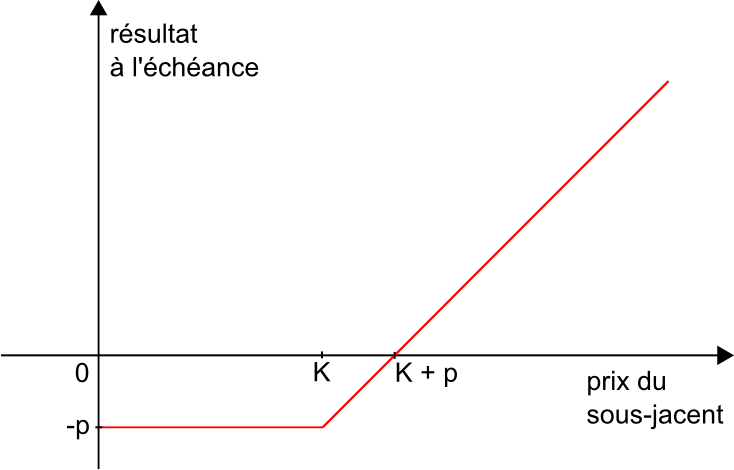
\includegraphics[scale=0.65]{Long_d'un_call.png}}
\subfloat[Short d'un call]{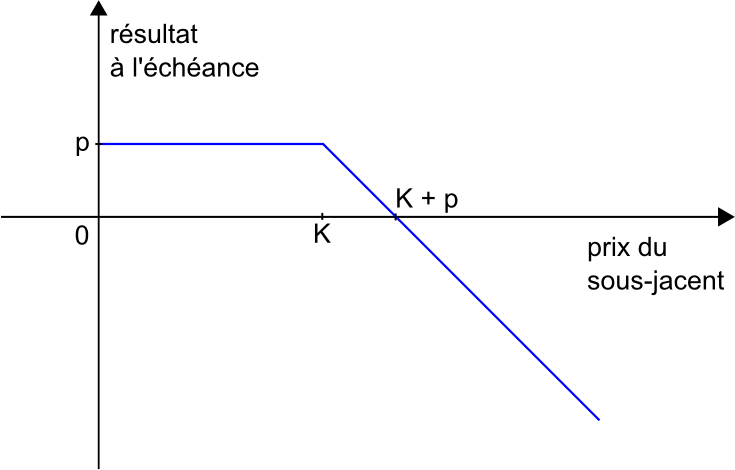
\includegraphics[scale=0.65]{Short_d'un_call.png}} \\
\subfloat[Long d'un put]{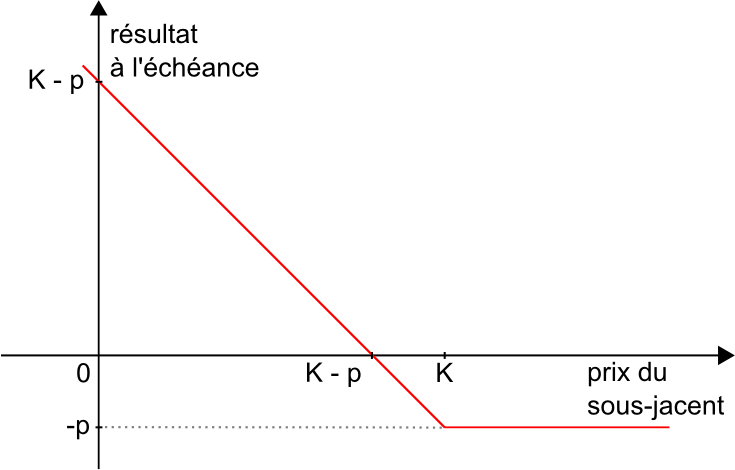
\includegraphics[scale=0.65]{Long_d'un_put.png}}
\subfloat[Short d'un put]{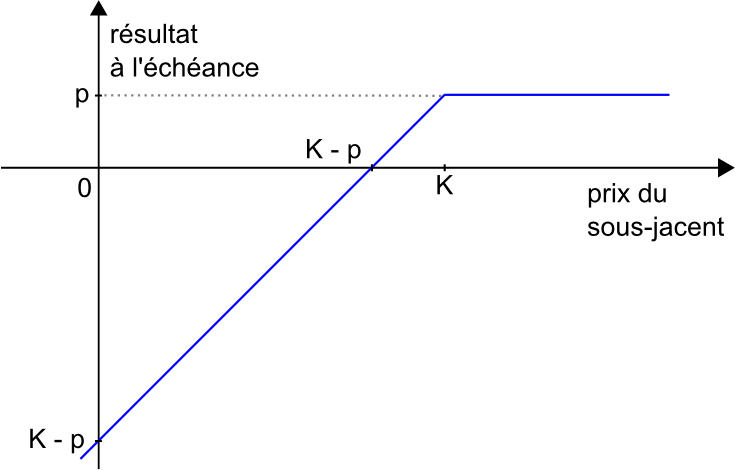
\includegraphics[scale=0.65]{Short_d'un_put.png}}
\caption{Evolution du prix de l'option}
\end{figure} 

\subsection{Modèle de Black-Scholes}
Ce modèle permet premièrement de pricer les options européennes (Europeean Call Option). On considère deux actifs : une option (bond/money market account) dont la valeur évolue continuement avec un intérêt fixé $r$ (rate) et une action (stock) dont le prix par unité (price per unit) est modélisé par un processus stochastique $(S_t, \hspace{1mm} t\geq 0)$.\\
On note $M_t$ le prix d'une unité de bond à l'instant $t$ en considérant $M_0=1$ on a $dM_t = rM_tdt$ soit $M_t= e^{rt}$. La première assertion du modèle de Black--Scholes est que $S$ satisfait l'équation différentielle stochastique suivante:
\begin{equation}
dS_t = S_t(\mu dt + \sigma dW_t)\hspace{2mm}\text{soit}\hspace{2mm}S_t=\exp{\bigg(\bigg(\mu - \frac{\sigma^2}{2}\bigg)t + \sigma W_t\bigg)}
\end{equation}
où $W$ représente un mouvement Brownien standard. $S$ représente donc un mouvement Brownian géométrique de paramètres $\mu$ et $\sigma$ (qui est nommée la \textit{volatilité} du prix).
\subsection{Modèle de Black-Scholes-Merton}

\subsubsection{Hypothèses}

Suite au krach de 1987, on trouve ci-après un modèle qui permet de prendre en compte les taux et les volatilités non constantes et qui permet de pricer des options qui payent des dividendes.
\\
On cherche à pricer un contrat européen, i.e. on cherche la fonction $P(t,X_t)$.
\\
\vspace{2mm}\\
\textbf{Hypothèse de non-arbitrage.} on suppose qu'il n'y a pas d'ooportunité d'arbitrage. i.e. il existe des processus $(a_t)$ et $(b_t)$ tels que 
\begin{align*}
    a_t X_t + b_t e^{rt} = P(t,X_t) \text{  pour  } 0 \leq t \leq T
\end{align*}

\subsubsection{Equation différentielle stochastique}

La propriété de self-financing nous donne
\begin{align*}
    d( a_t X_t + b_t e^{rt} ) = a_t dX_t + r b_t e^{rt} dt
\end{align*}
On a alors grace au lemme d'Ito,
\begin{align*}
    d( P(X_t, t)) = \bigg(\frac{\partial P}{\partial t} + \mu X_t \frac{\partial P}{\partial x} + \frac{1}{2}\frac{\partial^2 P}{\partial x^2} \sigma_t^2 \bigg) dt + \sigma \frac{\partial P}{\partial x} X_t dW_t
\end{align*}
donc en ré-injectant les deux équations,
\begin{align*}
   \bigg(\frac{\partial P}{\partial t} + \mu X_t \frac{\partial P}{\partial x} + \frac{1}{2}\frac{\partial^2 P}{\partial x^2} \sigma_t^2 \bigg) dt + \sigma \frac{\partial P}{\partial x} X_t dW_t = a_t dX_t + r b_t e^{rt} dt
\end{align*}
Soit,
\begin{align*}
   \bigg(\frac{\partial P}{\partial t} + \mu X_t \frac{\partial P}{\partial x} + \frac{1}{2}\frac{\partial^2 P}{\partial x^2} \sigma_t^2 \bigg) dt + \sigma \frac{\partial P}{\partial x} X_t dW_t = a_t \mu dt + r b_t e^{rt} dt + a_t \sigma X_t dW_t
\end{align*}
On peut alors identifier les termes en $dW_t$:
\begin{equation}
    a_t = \frac{\partial P}{\partial x}(t,X_t)
\end{equation}
On a alors avec la condition de non-arbitrage
\begin{equation}
    b_t = e^{-rt}(P(t,X_t)-a_t X_t) = e^{-rt}(P(t,X_t)- \frac{\partial P}{\partial x} X_t) 
\end{equation}
en ré-injectant dans l'équation de départ, on a en divisant par $dt$:

\begin{equation}
    \boxed{\frac{\partial P}{\partial t} + \frac{1}{2} \sigma ^2 {X_t}^2 \frac{\partial ^2 P}{\partial x^2} + r\bigg( X_t \frac{\partial P}{\partial x} - P\bigg) =0}
\end{equation}
C'est l'équation de Black-Scholes, qui est vérifiée pour chaque stock price $X_t$.
\\
\textbf{Exemple.} Pour pricer un European call option de strike $K$ et de maturité $T$, on a alors 
\begin{align*}
    \frac{\partial C}{\partial t} + \frac{1}{2} \sigma ^2 {S}^2 \frac{\partial ^2 C}{\partial S^2} + r\bigg( S \frac{\partial C}{\partial S} - C\bigg) =0
\end{align*}
Avec les conditions aux limites:
\begin{itemize}
    \item \textit{Expiration de l'option.} à $t=T$, $C(S,T)=(S-K, 0)_{+}$ car le prix de l'option est égal à la valeur intrinsèque, qui est la différence entre le prix de l'actif sous-jacent $S$ et le prix d'exercice $K$, si elle est positive, sinon, elle est nulle.
    \item \textit{Limite à l'infini.} Lorsque $S$ tend vers l'infini: $C(S, t) \rightarrow S$ car \textbf{le prix de l'option d'achat augmente à mesure que le prix de l'actif sous-jacent augmente}.
    \item \textit{Limite en 0.} Lorsque S tend vers zéro : $C(S, t) \rightarrow 0$ car le prix de l'option d'achat \textbf{ne peut pas être négatif}. 
\end{itemize}
Montrons que la solution de cette équation (prix d'un call européen sans dividendes) est:
\begin{align}
    C(S,t)=e^{-r(T-t)} N(d_2) \text{   avec   } d_2 = \frac{1}{\sigma \sqrt{T-t}}
\end{align}


\subsubsection{Parité call-put} entre un put et un call avec les memes maturity et strike price. On a tout d'abord,
\begin{align*}
    (S_T-K)_+ + (K-S_T)_- = S_T - K
\end{align*}
Il suffit alors d'appliquer des deux cotés de l'équation $e^{-r(T-t)} \mathbb{E}^{\mathbb{Q}}$ et on obtient
\begin{equation}
    C(t, S_t) - P(t, S_t) = S_t - K e^{-r(T-t)}
\end{equation}
Car $S_t$ est une martingale. 

\subsubsection{Dividendes}
On considère que lors d'une période de temps de $[t, t + d t]$ le paiement des dividendes s'écrit $qS_t dt$ avec $q$ constant.
Le sous-jaçent suit alors un mouvement brownien géométrique de dynamique:
\begin{equation}
    dS_t = (r-q)S_t dt + \sigma S_t dW_t^{\mathbb{Q}}
\end{equation}
On forme alors un portefeuille comme suit:
\begin{itemize}
    \item On long 1 call $C$
    \item On short $\Delta$ stock
\end{itemize}
On a alors 
\begin{equation}
    d \Pi_t = dC -\Delta dS_t - q\Delta S_t dt
\end{equation}
Avec la formule d'Ito on obtient:
\begin{equation}
   dV_t = \bigg(\frac{\partial V}{\partial t} + (r-q) S_t \frac{\partial V}{\partial S} + \frac{1}{2}\frac{\partial^2 V}{\partial S^2} \sigma_t^2 \bigg) dt + \sigma \frac{\partial V}{\partial S} S_t dW_t^{\mathbb{Q}} 
\end{equation}
L'absence d'opportunité d'arbitrage donne que la valeur du portefeuille sans-risque doit etre la meme que celle du portfeuille sans risque zéro-coupon i.e. $d\Pi_t = r\Pi_t dt$. En identifiant les termes en $dt$ et en $dW_t^{\mathbb{Q}}$, la forme modifiée de l'équation de Black-Scholes pour une option d'achat européenne avec des dividendes est la suivante :

\begin{equation*}
    \boxed{\frac{\partial C}{\partial t} + (r-q) S \frac{\partial C}{\partial x} + \frac{1}{2} \sigma ^2 {s}^2 \frac{\partial ^2 C}{\partial x^2}  - r C = 0}
\end{equation*}

 Le modèle de Black-Scholes nous permet d'écrire le prix d'un call $C$ et celui d'un put $P$:
\begin{equation}
    C(S,T) = e^{-qT}S_0 N(d_1) - e^{-rT}K N(d_2) \text{  et  }
    P(S,T) = e^{-rT}K N(- d_2) - e^{-qT}S_0 N(- d_1) 
\end{equation}
Dans ces équations, 
\begin{itemize}
    \item $S$ représente le prix actuel de l'actif sous-jacent, $S_0$ le prix initial
    \item $T$ représente la date d'échéance de l'option,
    \item $r$ représente le taux d'intérêt sans risque,
    \item $q$ représente le rendement attendu de l'actif sous-jacent,
    \item $K$ représente le prix d'exercice de l'option,
    \item $N$ est la fonction de répartition de la loi normale standard,
     on note $N$ (ou alors $\Phi$) la fonction de répartition de la loi Normale centrée réduite:
    \begin{align*}
     N(x) = \int_{-\infty}^{x} \frac{1}{\sqrt{2 \pi}} e^{- t^2 / 2} dt \hspace{3mm}\text{et}\hspace{3mm} N'(x) = \frac{1}{\sqrt{2 \pi}} e^{- x^2 / 2}
    \end{align*}
    \item $d_1$ et $d_2$ sont des variables qui dépendent de ces différents paramètres. sont utilisés pour calculer la probabilité que l'option soit exercée (ou non) à l'expiration. Plus précisément, $d_1$ mesure l'écart entre le prix actuel de l'actif sous-jacent et le prix d'exercice de l'option, ajusté pour prendre en compte les dividendes et la volatilité. D'autre part, $d_2$ mesure la même chose, mais sans prendre en compte les dividendes. 
    \begin{align*}
        d_1 = \frac{1}{\sigma \sqrt{T}} \ln{ \bigg[ \bigg( \frac{S}{K} \bigg) + \bigg( r-q + \frac{1}{2} \sigma^2 \bigg)T }\bigg] \hspace{3mm}\text{et}\hspace{3mm} d_2 = d_1 - \sigma \sqrt{T}
    \end{align*}
\end{itemize}
Et on peut calculer le prix le prix à terme (ou le prix modifié en avance) de l'actif sous-jacent $F$:
\begin{equation}
    F = e^{(r-q)T}S_0 
\end{equation}
 Ce modèle permet de calculer le prix d'une option en supposant que les mouvements du prix de l'actif sous-jacent suivent une marche aléatoire géométrique avec une volatilité constante. En d'autres termes, \textit{elle suppose que les rendements futurs de l'actif sous-jacent sont distribués de manière normale et que les investisseurs sont rationnels et ont des attentes homogènes concernant les rendements futurs}. Cette formule est largement utilisée dans la finance pour évaluer le prix des options, bien qu'elle ait ses limites et ses critiques.

\subsection{Le modèle binomial (Cox--Ross--Rubinstein)}
\subsubsection{Présentation}
Le modèle de Cox-Ross-Rubinstein (CRR) est une méthode de modélisation de la dynamique des prix des options d'achat \textit{call} et de vente \textit{put} dans le cadre de la théorie des options.
\vspace{2mm} \\
Le modèle CRR utilise une approche discrète pour décrire l'évolution des prix d'un actif sous-jacent. Il suppose que l'actif sous-jacent peut prendre deux valeurs distinctes à chaque période de temps. La variation de l'actif sous-jacent est représentée par un arbre binomial qui permet de calculer le prix de l'option à chaque période.
\vspace{2mm} \\
La formule CRR est particulièrement utile pour évaluer les \textit{options européennes}, qui peuvent être exercées uniquement à une date d'expiration spécifiée. Elle permet également de calculer les valeurs d'autres options complexes, comme les \textit{options américaines}, qui peuvent être exercées à tout moment avant la date d'expiration.
\subsubsection{Construction de l'arbre}
On part de la date à laquelle on souhaite valoriser l'option on finit à la date de d'expiration de l'option. A chaque étape, le sous-jacent augmente \textit{up} ou diminue \textit{down} en fonction d'un facteur spécifique $d$ ou $u$ (avec $u\geq 1$ et $0<d\leq 1$). Si $S$ est le prix actuel, alors le prix au pas suivant sera $S_u = S\times u$ ou $S_d = S\times d$. Les facteurs spécifiques sont calculés en prenant en compte la \textit{volatilité} $\sigma$ du sous-jacent, le pas de temps $t$ (en année, selon la convention du nombre de jours du sous-jacent). En considérant que $V(\log S)=\sigma ^2 t$, on a:
\begin{equation}
    u=e^{\sigma \sqrt{t}}\hspace{3mm} \text{et} \hspace{3mm} d=e^{- \sigma \sqrt{t}} = \frac{1}{u}
\end{equation}
 La méthode CRR assure le fait que l’arbre est recombinant, i.e. si les mouvements du sous-jacent sont d’abord une augmentation puis une diminution, le prix sera le même que si les mouvements suivis avaient été d’abord une diminution puis une augmentation. Dans ce cas là, les deux branches fusionnent et se recombinent. Cette propriété réduit donc le nombre de nœuds de l’arbre et par conséquent accélère le calcul du prix de l’option. Cette propriété permet également de calculer la valeur de l’actif sous-jacent à chaque nœud directement par des formules, sans passer par la création d’un arbre. La valeur d’un nœud est donc $S_n = S_0 \times u^{N_u - N_d}$
 \subsubsection{Calcul de la valeur de l'option sur les noeuds}
 \textbf{Calcul pour chaque noeud final.} La valeur de l'option est sa valeur intrinsèque i.e.
 \begin{itemize}
     \item $\max[ (S-K), 0]$ pour un call 
     \item $\max[ (K-S), 0]$ pour un put
 \end{itemize}
 Où $K$ est le strike (prix d'exercice de l'option) et $S$ est le spot (cours au comptant) du sous-jacent.
 \hspace{2mm} \\
 \textbf{Calcul pour les noeuds antérieurs.} La valeur de l'option pour chaque noeud est trouvée en utilisant la valeur du noeud précédent, en remontant vers le premier noeud de l'arbre (i.e. la valeur de l'option à la date ou l'on souhaite la valoriser).
\vspace{2mm}
     En prenant en compte l’hypothèse de neutralité du risque, le prix, aujourd’hui, d’un instrument dérivé est égal à la valeur de ses bénéfices futurs actualisés en fonction du taux sans risque. Par conséquent, la valeur attendue est calculée en utilisant la \textbf{valeur de l’option lors des deux derniers nœuds} (appelés ici option \textit{up} et option \textit{down}) pondérés par leurs probabilités respectives. Soient $p$ la probabilité d’une variation à la hausse de la valeur du sous-jacent et $(1-p)$ la probabilité d’une variation à la baisse. La valeur de l’option est ensuite actualisée avec $r$ le taux sans risque correspondant à la durée de l’option.
     \begin{equation}
         C_{t-\Delta t,i} = e^{-r\Delta t} \bigg( pC_{t,i+1} + (1-p)C_{t, i-1} \bigg)
     \end{equation}
     Où $C_{t,i}$ représente la valeur de l'option pour le $i$-ème noeud au temps $t$, $p$ représente la probabilité de la loi binomiale qui simule le mouvement brownien géométrique de l'action sous-jacente avec les paramètre $r$ et $\sigma$ et $q$ est le rendement du dividende du sous-jacent correspondant à la durée de vie de l’option i.e.
     \begin{align*}
         p = \frac{e^{(r-q)\Delta t}-d}{u-d} 
     \end{align*}
     Pour qu'on ait $p<1$, il faut avoir $\Delta t < \frac{\sigma ^2}{(r-q)^2}$. \\

     $C_{t-\Delta t, i}$ représente le juste prix du dérivé à un point donné dans le temps (c’est-à-dire chaque nœud), étant donné l’évolution du prix du sous-jacent à ce point. C’est la valeur de l’option à ce point – opposée à la valeur d’exercice. 


 \subsubsection{Exemple d'utilisation}
 L'exemple d'utilisation du code affiche l'arbre de prix pour un actif sous-jacent initial de 100, un prix d'exercice de 110, un taux d'intérêt sans risque de 5\%, une durée de vie de l'option de 1 an, 3 périodes de temps dans l'arbre et une volatilité de 20\%.
\begin{lstlisting}[language=Python]
import numpy as np

# Fonction pour calculer l'arbre de Cox-Ross-Rubinstein
def CRR_tree(S0, K, r, T, N, sigma):
    dt = T / N
    u = np.exp(sigma * np.sqrt(dt))
    d = 1 / u
    p = (np.exp(r * dt) - d) / (u - d)
    # Initialisation de l'arbre
    tree = np.zeros((N + 1, N + 1))
    for i in range(N + 1):
        for j in range(i + 1):
            tree[j, i] = S0 * (u ** (i - j)) * (d ** j)
    return tree

# Fonction pour afficher l'arbre de Cox-Ross-Rubinstein
def print_tree(tree):
    N = tree.shape[0] - 1
    for i in range(N + 1):
        print(' ' * (N - i), end='')
        for j in range(i + 1):
            print('{0:8.2f}'.format(tree[i - j, j]), end='')
        print()
\end{lstlisting}
Voici ce que retourne le code:
\begin{lstlisting}[language=Python]
S0 = 100
K = 110
r = 0.05
T = 1
N = 3
sigma = 0.2

tree = CRR_tree(S0, K, r, T, N, sigma)
---------------------------------------
[in] > print_tree(tree)
[out]
           100.00
      0.00       112.24
     0.00      89.09  125.98       
    0.00    0.00  100.00  141.40
\end{lstlisting}

\subsection{PDF du prix et formule de \textsc{Breeden--Litzenberger}}

On cherche à calculer la densité de probabilité du prix. \textsc{Breeden--Litzenberger} (1978) ont montré le lien entre la dérivée de la formule de \textsc{Feynmann--Kac} et la densité du prix.

\begin{theorem}
    
\end{theorem}

\section{Autres modèles de pricing}

On cherche alors à introduire issus de Black-Scholes mais qui incluent des termes correctifs pour tenter de modéliser au mieux le comportement réels de la volatilité implicite observée sur le marché. On distingue alors deux types de modèles, ceux à volatilité "locale" et ceux à volatilité stochastique. \textit{Les modèles à volatilité locale ont l'avantage de conserver l'aspect de marché complet car ceux-ci n'introduisent pas, à la dfférence des modèles à volatilité stochastique, de dynamique supplémentaire dans la modélisation. L'inconvénient vient du fait que les dynamiques des volatilités implicites observés dans le marché ne sont pas en adéquation avec les dynamiques prévues dans le modèle} \cite{ENS} La complétude du marché signie qu'on peut identier chaque source d'aléa
par un portefeuille de produit. Autrement dit on peut se couvrir ou isoler
chaque source de risque. Cette complétude des marchés ne peut être conservée qu'en introduisant des produits comme le VIX ou les variances forward qui apportent une méthode supplémentaire de couverture

\subsection{Evaluation de la volatilité}

\subsubsection{Modèle GARCH(1,1)}

\subsubsection{Modèle GARCH(1,1)}

\subsubsection{Volatilité Implicite}

Dans le modèle de Black--Scholes, la volatilité est considérée comme constante. La volatilité implicite est alors définie pour refleter la perception du marché quant à la fluctuation future des prix d'un actif sous-jacent. Contrairement à la volatilité historique, qui se base sur les mouvements passés des prix, la volatilité implicite est déduite du prix actuel des options. Mathématiquement, la volatilité implicite (\(\sigma_{\text{implicite}}\)) est souvent déterminée en inversant la formule de prix de l'option. Pour une option d'achat européenne, par exemple, la formule de Black-Scholes est souvent utilisée :

\begin{equation}
C = S_0 N(d_1) - Xe^{-rT}N(d_2)
\end{equation}

où :
\begin{align*}
d_1 &= \frac{\ln\left(\frac{S_0}{X}\right) + \left(r + \frac{\sigma_{\text{implicite}}^2}{2}\right)T}{\sigma_{\text{implicite}}\sqrt{T}} \\
d_2 &= d_1 - \sigma_{\text{implicite}}\sqrt{T}
\end{align*}

Dans ces équations, \(C\) est le prix de l'option d'achat, \(S_0\) est le prix actuel de l'actif sous-jacent, \(X\) est le prix d'exercice de l'option, \(r\) est le taux d'intérêt sans risque, \(T\) est le temps restant jusqu'à l'expiration de l'option, et \(N\) est la fonction de distribution cumulative de la loi normale standard.
\vspace{2mm}
Inverser cette équation pour résoudre \(\sigma_{\text{implicite}}\) donne une estimation de la volatilité implicite basée sur le prix actuel de l'option et d'autres paramètres du marché.

\begin{figure}[H]
    \centering
    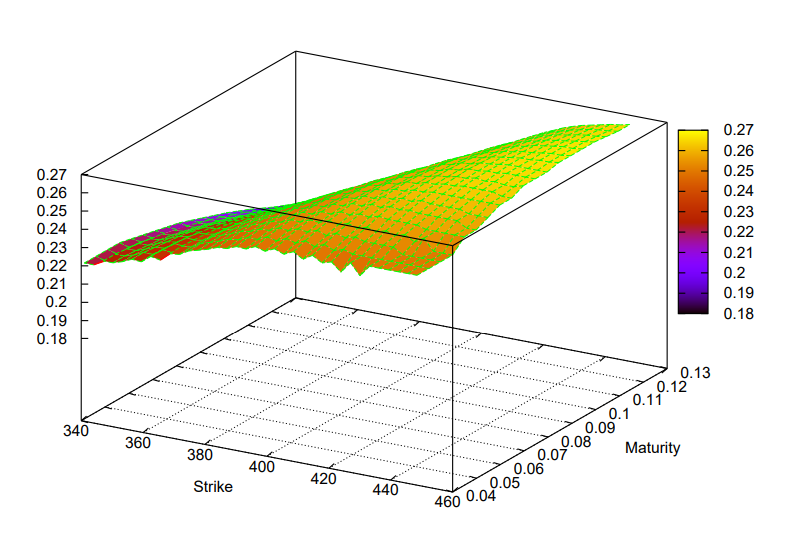
\includegraphics[scale=0.7]{implied_vol.png}
    \caption{The volatility surface}
    \label{fig:enter-label}
\end{figure}

On constate sur les données de marché que la volatilité implicite ne peut être considérée comme constante. Elle dépend du strike et de la maturité. On peut alors supposer plusieurs dynamiques afin de modéliser au mieux la volatilité implicite face aux données de marché. On peut par exemple supposer qu'elle suit une dynamique stochastique propre, avec un brownien corrélé au brownien du sous-jaçent. De plus, les phénomènes exeptionels tels que les krachs ou les défauts font présenter des queues de distributions plus épaisses et imposent une distribution non gaussienne (kurtosis positif). 


\subsection{Modèle de volatilité locale}

Dans les modèles à volatilité locale, la volatilité est une fonction non plus constante comme dans Black-Scholes, mais une fonction du temps et du spot $S_t$. La dynamique du sous-jaçent devient alors
\begin{equation*}
    dS_t = \mu S_t dt + \sigma(t, S_t) dB_t
\end{equation*}
Dans le modèles de Black-Scholes, la fonction de volatilité est une fonction affine de $S_t$ avec $\sigma$ constant pour chaque option (chaque strike et chaque maturité). On distingue deux modèles de volatilité locale, la volatilité de Dupire, où la fonction de volatilité est explicite, et le modèle CEV (Constant Elasticity of Variance) où la fonction de volatilité n'est pas explicite.
\subsubsection{Volatilité de Dupire}

Dans ce modèle, la volatilité est construite afin de calibrer au mieux le smile (volatilité implicite en fonction du strike).
\begin{figure}[H]
    \centering
    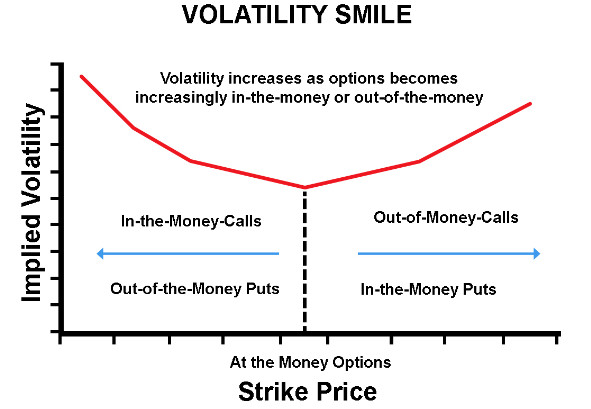
\includegraphics[scale=0.5]{volatility-smile.png}
    \caption{Smile de la volatilité implicite}
    \label{fig:enter-label}
\end{figure}
Afin de simplifier le modèle, on considère que les taux sont nuls et que donc la dynamique de $S_t$ est
\begin{equation*}
    dS_t = \sigma (t, S_t) dB_t
\end{equation*}
On définit alors la fonction $\sigma$ comme la \textbf{projection markovienne} de la dynamique de $S_t$:
\begin{equation}
    \sigma (t, S_t) = \sqrt{ \mathbb{E} \bigg[ \frac{d\langle S_t \rangle}{dt} \bigg| S_t = S \bigg] }
\end{equation}

En écrivant le prix d'un call $C(T,K) = \mathbb{E}_Q [(S_T - K)_+]$ sous la forme intégrale et en dérivant par rapport à la maturité on obtient

\begin{equation*}
    \frac{\partial C(T,K)}{\partial T} = \int_{K}^{+\infty} (x-K)_+ \frac{\partial v(dx)} {\partial T} \label{dupire}
\end{equation*}
Avec $v(dx)$ la densité de probabilité du prix $S_t$. On pose la fonction $f$ qui associe à chaque pay-off $h(S_T)$ son prix $\mathbb{E}[h(S_T)|S_t = x] = f(x, t)$. On écrit alors l'espérance conditionelle et on obtient:
\begin{equation*}
    \mathbb{E}[h(S_T)] = \mathbb{E}\bigg[\mathbb{E}[h(S_T)|S_T = x]\bigg] = \int f(x,t) v_t (x)dx 
\end{equation*}
Le terme de gauche ne dépend pas de $t$, alors en dérivant l'équation par raport à $t$ il vient

\begin{equation*}
    \int \frac{\partial f(x,t)}{\partial t} v_t (x)dx + \int f(x,t) \frac{\partial v_t (x)}{\partial t} dx = 0
\end{equation*}

En appliquant la formule d'Ito à $f$ on obtient

\begin{equation*}
    \frac{\partial f(x,t)}{\partial t} + \frac{1}{2} \sigma^2 (x,t)x^2 \frac{\partial^2 f(x,t)}{\partial x ^2} = 0
\end{equation*}
Après intégration par parties on peut réecrire cette relation en fonction de $f(x,t)$. On obtient alors que pour tout $f$ issu de tout pay-off $h(S_T)$ on a:
\begin{equation*}
    \int \bigg( \frac{1}{2} \frac{\partial^2}{\partial x^2} (\sigma^2x^2v) - \frac{\partial v_t(x)}{\partial t} \bigg) f(x,t)dx = 0
\end{equation*}
Il vient alors la relation
\begin{equation*}
    \frac{1}{2} \frac{\partial^2}{\partial x^2} (\sigma^2x^2v) = \frac{\partial v_t(x)}{\partial t}
\end{equation*}
En injectant ce résultat dans \eqref{dupire} on obtient alors
\begin{align*}
    \frac{\partial C(T, K)}{\partial T} &= \int_{K}^{+\infty} (x-K)_+ \frac{\partial v(dx)} {\partial T} \\
    &= \frac{1}{2} \int_{K}^{+\infty} (x-K)_+ \frac{\partial^2}{\partial x^2} (\sigma^2x^2v) \\
    &= \frac{1}{2} \sigma ^2 (T,K) K^2 v_T(K) \\
    &= \frac{1}{2} \sigma ^2 (T,K) K^2 \frac{\partial ^2 C(T,K)}{\partial K^2}
\end{align*}
On a supposer que $\sigma^2 x v$ admet une asymptote à l'infini qui est nulle afin de pouvoir calculer l'intégrale (???). On obtient alors la formule de volatilité de Dupire

\begin{theorem}[Formule de volatilité de Dupire]
Dans le cadre du modèle de volatilité locale de Dupire, on a la relation entre la volatilité et le prix du call à une maturité $T$ et un strike $K$ donné dans le cas où le taux d'intéret $r_t$ est nul:
\begin{equation}
    \sigma ^2(T,K) = \frac{2 \frac{\partial \mathbb{E}[(S_T - K)_+]}{\partial T}}{K^2 \frac{\partial^2 \mathbb{E}[(S_T - K)_+]}{\partial K^2}}
\end{equation}
\end{theorem}
\subsubsection{Constant Elasticity of Variance Model (modèle CEV)}
Le modèle CEV, introduit dans [3], est un cas particulier de modèle à
volatilité locale. Il suppose l'existence d'une forme particulière de volatilité et donc de dynamique du sous-jacent. L'intérêt de ce modèle est l'existence de formules approchées et de méthode de calibration qui en font un très bon modèle proxy. Un modèle proxy est un modèle de première approximation qu'on enrichit ensuite à l'aide de méthode de perturbation.
La dynamique du modèle s'écrit:
\begin{equation}
    dS_t = \sigma S_t ^{\gamma} dW_t
\end{equation}
$\sigma$ représente la volatilité initiale et on peut jouer aussi sur le paramètre $\gamma$, qui est pris en générale entre 0 et 1.
\subsection{Modèle de volatilité stochastique}

\subsubsection{Modèle de Heston}

\subsubsection{Stochastic Alpha, Beta, Rho model (modèle SABR)}

\subsubsection{Modèle de Bergomi}

\section{Dérivés de taux}
Un \textbf{interest rate option} ou option sur taux d'intéret, donne au \textit{holder} le droit (mais pas l'obligation) donne le droit à l'acheteur d'emprunter un montant déterminé (Cap) ou d'en prêter un (Floor) à un taux d'intérêt fixé (taux d'intérêt d'exercice) pour une durée spécifique. On distingue plusieurs types:
\begin{enumerate}[label=\textit{(\roman*)}]
    \item \textbf{Cap option} Elle donne le droit au \textit{holder} de recevoir un paiement si le taux d'intéret dépasse un certain montant fixé à l'avance.
    \item \textbf{Floor option} Elle donne le droit au \textit{holder} de recevoir un paiement si le taux d'intéret passe en dessous un certain montant fixé à l'avance.
    \item \textbf{Collar option} Correspond à une combinaison d'achat de cap et de vente de floor (ou inversemment) permettant d'encadrer le taux d'intéret.
\end{enumerate}

\subsection{Zero-coupon bond}

Le prix $B$ d'un bond et le yield $y$ sont reliés par la formule suivante. On suppose que le bond rémunère au detenteur un cash flow $c_i$ au temps $t_i$ pour $(0\leq i\leq n)$
\begin{equation}
    B = \sum_{i=1}^{n} c_i e^{-yt_i}
\end{equation}
On définit alors la \textbf{duration} du bond par la relation:
\begin{equation}
    D = \frac{1}{B} \sum_{i=1}^{n} c_i e^{-y t_i} = \sum_{i=1}^{n} t_i \bigg( \frac{ c_i e^{-y t_i} }{B}\bigg)
\end{equation}
Le prix du bond peut etre aussi exprimé comme la somme de tous les futures coupons et de la valeur nominale, et le yeild à maturité $y_n$
\begin{equation}
    P = \sum_{i=1}^{n} \frac{c_i}{(1+y_n)^i}+\frac{\text{FV}}{(1+y_n)^n}
\end{equation}
On peut essayer de trouver une relation entre la variation du prix du bond et celle du yield comme suit.
\begin{equation}
    dP = \bigg[ \sum_{i=1}^{n} \frac{-ic_i(1+y_n)^{i-1}}{(1+y_n)^{2i}}+\frac{n \text{FV}(1+y_n)^{n-1}}{(1+y_n)^{2n}} \bigg]dy_n = \frac{-D P dy_n}{1+y_n}
\end{equation}
On définit la \textit{modified duration} $D^*$ comme la duration divisée par $1+y_n$. On obtient alors la relation 
\begin{align*}
    \frac{dP}{P} = -D^* dy_n
\end{align*}
En supposant que le yield suit un modèle log-normal $dy_n = y_n \sigma_y dW_t$, On obtient alors la relation vérifiée par le prix du bond $P$,
\begin{equation*}
    \frac{dP}{P} = - \sigma_y D^* y_n dW_t
\end{equation*}
$D$ est \textbf{l'élasticité} du prix de l'obligation par rapport à l'interest rate.
\begin{equation*}
    D = -\frac{d(\log P)}{d(\log 1+r)}
\end{equation*}
Pour évaluer le prix d'une obligation en pratique, on utilise la relation, dans le cas de coupon fixes (Fixed Income)
\begin{equation}
    \boxed{P = c \text{FV} \times \frac{1-(1+r)^{-n}}{r} + \frac{\text{FV}}{(1+r)^n}}
\end{equation}
Ou
\begin{itemize}
    \item $\text{Coupon} = \text{Par Value} \times \text{Coupon Payment}$
    \item $r$ désigne le \textit{rate of return}
    \item $n$ désigne le nombre de \textit{years to maturity} dans le cas de \textit{annual coupon paying bonds}
\end{itemize}


\subsection{Short rate models}
Le SRM donne une dynamique pour le \textit{interest rate} de la forme:
\begin{equation*}
    dr = \alpha (t,S_t) dt + \beta (t,S_t) dW_t
\end{equation*}

\subsubsection{Modèle de Cox-Ingersoll-Ross}
Un exemple de \textit{short rate model} est le modéle de \textsc{Cox--Ingersoll--Ross} model. Il est utilisé lors du pricing d'un \textit{interest rate derivative}. La dynamique est de la forme:
\begin{equation*}
    dr_t = a(b-r_t)dt + \sigma \sqrt{r_t}dW_t
\end{equation*}
Le \textit{drift} est composé de deux paramètres $a$ et $b$ qui peuvent etre interprétés par $a$ le \textit{speed of adjustement} à la moyenne $b$. Pour éviter d'avoir des valeurs négative on a aussi la \textbf{Condition de Feller}
\begin{align*}
    2ab \geq \sigma ^2
\end{align*}

\subsubsection{Modèle de Hull--White}

\subsubsection{Modèle de Vasicek}
\textbf{Définition.} Un processus d'Orstein--Uhlenbeck est un processus stochqstique vérifiant l'équation différentielle stochastique
\begin{equation}
    dX_t = -\theta (S_t - \mu) dt + \sigma dW_t
\end{equation}
Ou $\sigma$, $\mu$ et $theta$ sont déterministes.
\\
\vspace{0.5mm} \\
Pour résoudre cette équation, on peut appliquer le lemme d'Itô à la fonction $f(t, X_t) = X_t e^{\theta t}$. Il vient 
\begin{align}
    df(t, X_t) = \theta X_t e^{\theta t} + e^{\theta t}dX_t = \theta \mu  e^{\theta t} dt + \sigma e^{\theta t}dW_t
\end{align}
On obtient alors 
\begin{align}
    X_t = X_0 + \mu \theta \int_{0}^{t} e^{\theta s}ds + \sigma  \int_{0}^{t} e^{\theta s}dW_s
\end{align}
On peut montrer que
\begin{enumerate}[label=\textit{(\roman*)}]
    \item \[\mathbb{E}[X_t] = X_0e^{- \theta t} + \mu (1-e^{\theta t}) \]
    \item \[Var(X_t)=\frac{\sigma^2}{2\theta} e^{-2\theta t}(e^{2\theta t} -1)  \]
    \item \[Cov(X_t,X_s) = \frac{\sigma^2}{2\theta} e^{-\theta(s+t)}(e^{2\theta \min{(s,t)}} -1) \]
\end{enumerate}

\subsection{Health--Jarrow--Morton framework}

\subsection{Market models}
Le market model est utilisé pour les quantités observables telles que les \textbf{forward rates} ou encore les \textbf{swap rates}. Par exemple le modèle \textsc{Libor} (London Interbank Offered Rate) donne la dynamique pour le $j$-ème forward rate $f_j$:
\begin{equation*}
    \frac{df_j}{f_j} = \mu_j dt + \sigma_j dW_t^{(j)}
\end{equation*}



\subsection{Markov functional models}

\section{Dérivé Action (EQD)}

\subsection{Les types de dérivés sur action}

\subsubsection{Les options et warrants}

Un call warrant (put warrant) sur actions donne à son acquéreur le droit et non l’obligation d’acheter (de vendre) lesdites actions à un prix d’exercice convenu à l’avance et ceci à tout moment d’ici l’échéance prévue au contrat.

Mais les warrants sur actions se distinguent des options sur actions sur un certain nombre de points :
\begin{itemize}
    \item Les warrants sont des \textbf{valeurs mobilières (securities)}, créées par un émetteur \textbf{(établissement financier)} pour être proposées à la vente aux investisseurs, alors que les options sont des \textbf{contrats (derivative)}, créés par une entreprise de marché \textbf{(Euronext par exemple)}, s’agissant des options échangées sur un marché organisé ou par des établissements financiers s’agissant des options OTC. Les warrants figurent sur le même compte titres que les actions, tandis que la négociation d’options donne lieu à la création d’un compte distinct ;

    \item Leurs caractéristiques (échéances, prix d’exercice, quotités) sont choisies par l’émetteur alors que celles des options sont standardisées ;

    \item Les warrants sont de type \textbf{américain} (on peut les exercer à tout moment entre la date d’achat et la date d’échéance) alors que les options peuvent être de type \textbf{américain ou européen.}

    \item Un nombre illimité d’options peut être créé pour une même classe mais le nombre de warrants émis sur une maturité et un prix d’exercice donnés est en revanche limité ;

    \item Si les options peuvent être négociées à l’unité, il y a souvent une taille minimale de transaction sur les warrants. Exemple : si cette taille minimale est de 1000 unités, on ne peut acheter ce warrant que par multiple de 1000 ;

    \item La liquidité des warrants (proposition permanente de prix à l’achat et à la vente) est généralement assurée par le seul émetteur alors que plusieurs établissements « teneurs de marché » proposent généralement des prix dans le cas des options. \textbf{Lorsque tous les warrants déjà émis sont aux mains des investisseurs et que l’émetteur ne souhaite pas en émettre de nouveaux, il ne peut donc coter que des prix à l’achat (« bid only ») ;}
\end{itemize}
\subsubsection{Les Turbos}

L’élément essentiel du Turbo est la \textbf{barrière désactivante (knock out)} ou « seuil de sécurité ». Lorsque le cours de l’actif sur lequel est basé le Turbo atteint ce seuil, le Turbo est immédiatement « désactivé », c’est-à-dire qu’il est radié de la cotation. Il ne peut plus être échangé. Dans le cas des Turbos « classiques », il perd alors toute valeur. Les Turbos « classiques » ont une durée de vie fixée à l’avance : la maturité. Les Turbos Infinis / Illimités n’ont pas de date d’échéance, ils ont une durée de vie infinie.

\subsubsection{Les Compo et Quanto}

Ici, la devise utilisée dans l'option est différente de celle du sous-jaçent. Le produit est donc exposé au risque de change. Le payoff pour ces deux produits est
\begin{equation*}
    QC = FX_0 max(S_T - K, 0)
\end{equation*}
Ce qui distingue le compo du quanto est 

\subsubsection{Les futures contracts}

Le future (contrat à terme en français) est un contrat par lequel deux parties s’engagent à acheter (ou vendre) \textbf{une quantité déterminée d’un action}, à une date d’échéance et à un prix convenus à l’avance. Il permet d’anticiper les variations futures d’un actif sous-jacent et peut donc servir à couvrir un portefeuille contre les fluctuations à venir du marché. Il permet aussi de dynamiser les performances de son portefeuille. Le future constitue un engagement ferme, il doit être exécuté à sa date d’échéance par ses contreparties : l’acheteur du future doit acheter l’actif sous-jacent au prix convenu et le vendeur doit livrer l’actif.

\subsubsection{Les obligations convertibles}

Une obligation convertible est un prêt qui, à son terme, peut être remboursé soit en actions de l’entreprises, soit en numéraire. Elle s’apparente donc à une option d’achat sur les actions.
\vspace{2mm}
Ce mécanisme de financement permet à des investisseurs qui ne souhaitent pas prendre le risque d’entrer immédiatement au capital d’une entreprise de tout de même bénéficier du développement de celle-ci.

\subsubsection{Les Equity Swaps}

Les equity swaps sont des produits OTC. Ils permettent notamment 
\begin{itemize}
    \item \textbf{couvrir contre une baisse probable à court terme d’un portefeuille d’actions.} Le système permet ainsi d’éviter les impacts négatifs sur le court terme sans pour autant devoir vendre le portefeuille d’actions jugé rentable sur le long terme.  
    
    \item à un investisseur qui n’a pas légalement la possibilité d’acquérir un stock de \textbf{bénéficier de son rendement tout en respectant les restrictions légales}.
    
    \item Bénéficier de la performance d’un actif sans forcément acquérir l’actif en question, ce qui peut parfois être pratique pour des titres assez chers.
\end{itemize} 
\textbf{Hedge d'un equity swap.} Un investisseur peut, au lieu d’acheter des stocks directement sur le marché, passer par un \textbf{prime broker}. Dans ce cas, il va traiter un total return swap avec son prime broker qui lui paiera la performance des stocks et recevra en contrepartie les intérêts d’un taux flottant (floating rate). Afin de se couvrir, le prime broker va alors acheter les stocks et les détenir physiquement pour couvrir le risque de marché lié aux variations des prix du stock. 

\vspace{2mm}

\textbf{Exemple.} 
Prenons l’exemple d’un prime broker qui va conclure un contrat price return swap pour payer la performance de N stocks A et recevoir les intérêts d’un nominal N.  

Sur la période du swap, pour des raisons de simplicité, considérons l’absence de tombée de dividendes sur le stock A, et que le swap a une seule période entre t0 et t1.  
Le taux associé à la floating leg à l’issue de la période étant r1, S0 le spot du stock A à t0 et S1 le spot du stock A à t1. 

À $t_0$ :
\begin{itemize}
    \item Flux sur la floating leg: $0$ 
    \item Pour se hedger, le prime broker achète $n$ stocks A au prix unitaire $S_0$, le flux associé à cette transaction : $-n S_0$ 
\end{itemize}
À $t_1$ : 
\begin{itemize}
    \item Flux sur la floating leg: $N r_1$ 
    \item Flux sur la performance leg : le prime broker paie la performance des stocks sur la période $–n (S_1-S_0)$ 
    \item Le prime broker solde sa position sur les stocks détenus et reçoit donc $n*S_1$ 
\end{itemize}
À la maturité du swap, le total $T$ des flux financiers payés et reçus par le prime broker :  
\begin{equation}
    T = -n S_0 + N r_1 - n (S_1-S_0) + n S_1 = N r_1     
\end{equation}
Le prime broker est donc couvert contre les fluctuations du prix du stock et reçoit sans risque les intérêts du nominal N. 

\subsection{Réplication d'une option digitale}

On peut répliquer une option digitale de strike K à l'aide de positions short et long d'un call option de strike K. 

Pour cela il suffit de 
\begin{itemize}
    \item Long 1 call de maturité $K$
    \item Short $\delta$ call de maturité $K+\delta$ et de faire tendre $\delta$ vers 0 pour etre le plus proche possible de l'option digitale
\end{itemize}
\begin{figure}[H]
    \centering
    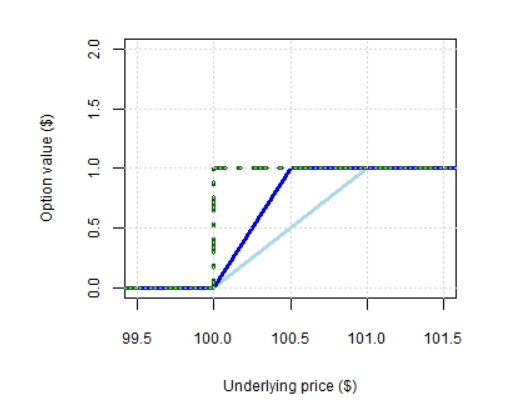
\includegraphics{replicating.png}
    \caption{replication d'une digital avec 1 call de maturité $100+1$ (bleu clair) et 0.5 call de maturité $100+0.5$ (bleu marine)}
    \label{fig:enter-label}
\end{figure}

\subsection{Evaluation d'un contrat forward et future}

\subsubsection{Prix d'un future -- Arbitrage \textit{cash and carry}}



\subsubsection{Prix d'un forward}
\subsubsection{Détermination sous Black--Scholes}

\subsection{Les Greeks}

 les grecques (ou "greek letters" en anglais) font référence à un ensemble de paramètres qui mesurent la sensibilité d'un instrument financier, tel qu'une option, à certains facteurs de risque, tels que la volatilité, les taux d'intérêt ou les mouvements du sous-jacent. Elles sont très utiles pour les traders et les investisseurs car ils leur permettent de comprendre les risques et les opportunités associés à un instrument financier donné, ainsi que de concevoir des stratégies de couverture et d'optimisation de leur portefeuille. En reprenant le modèle de Black-Scholes
 Et les paramètre $d_1$ et $d_2$ qui représentent

 On utilise le développement en série de Taylor (à l'ordre 2) pour faire apparaitre les \textit{sensitivities} i.e.
 \begin{equation}
     \Delta V = \frac{\partial V}{\partial S} \Delta S + \frac{\partial V}{\partial T} \Delta T + \frac{\partial V}{\partial \sigma} \Delta \sigma + \frac{\partial V}{\partial r} \Delta r + \frac{1}{2}\frac{\partial^2 V}{\partial S ^2} (\Delta S)^2
 \end{equation}

On peut identifier les principales Greeks dans le tableau, voici les détails de chacune d'entre elles

\begin{table}[]
    \centering
 \begin{tabular}{|c||c|c|c|}
      \hline
     Greek & Expression & Exposition & Définition \\
     \hline
     Delta & $\Delta = \frac{\partial V}{\partial S}$ & Actif & variation du SJ \\
     \hline
     Gamma & $\gamma = \frac{\partial V^2}{\partial^2 S}$ & Convexité du payout & variation du Delta \\
     \hline
     theta & $\theta = \frac{\partial V}{\partial T}$ & Temps & temps \\
     \hline
     rho & $\rho = \frac{\partial V}{\partial r}$ & interest rate & RFR \\
     \hline
     vega & $ \vartheta = \frac{\partial V}{\partial \sigma}$ & volatilité &  vol \\
     \hline
     volga & $ \frac{\partial V^2}{\partial^2 \sigma}$ & vol de vol & vol de vol \\
     \hline
     vanna & $ \frac{\partial V^2}{\partial \sigma \partial S}$ & Skew & var de delta (vol) ou vega (SJ) \\
     \hline
 \end{tabular}
 \caption{Résumé des principales Greeks}
\label{tab:my_label}
\end{table}
 \subsubsection{Le delta $\delta$}
 \textbf{Delta is the first-order sensitivity of the price to a movement in the spot price, S.}
 Le delta d'une option mesure la sensibilité de son prix à une variation donnée du cours du sous-jacent.
 \begin{align*}
     \delta = \frac{\partial P}{\partial S}, \hspace{2mm} \delta_{call} = N(d_1), \hspace{2mm} \delta_{put} = \delta_{call} - 1 = N(d_1) - 1
 \end{align*}
La prime d'un \textit{call} est une fonction croissante du prix du sous-jacent, $\delta_{call} \geq 0$, alors que celle d'un \textit{put} en est une fonction décroissante, $\delta_{put} \leq 0$. En effet, plus le prix du sous-jacent est élevé, plus la probabilité que le call soit dans la monnaie est grande. Symétriquement, plus le prix du sous-jacent est bas, plus la probabilité que le put soit dans la monnaie est grande. Ainsi, lorsqu'une option a un delta égal (en valeur absolue) à ou proche de 0,5, on dit qu'elle est à la monnaie. 
\begin{figure}[H]
    \centering
    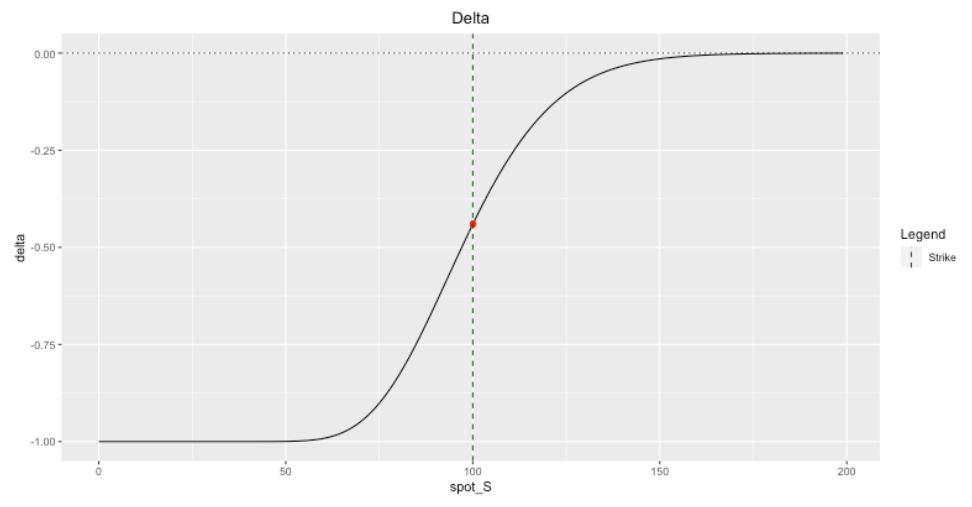
\includegraphics[scale=0.6]{delta.png}
    \caption{Evolution du $\Delta$ en fonction du spot price $S$}
    \label{fig:enter-label}
\end{figure}

\textbf{Delta Hedging} Le Delta Hedging permet de se couvrir d'une position 
\subsubsection{Le gamma $\gamma$}
\textbf{Gamma measures the change in delta due to the change in underlying price}. Le gamma représente la convexité ou la termaxité du prix d'une option en fonction du cours du sous-jacent.
\begin{align*}
    \gamma_{call} = \gamma_{put} = \frac{\partial ^2 P}{\partial S ^2} = \frac{N'(d_1)}{S \sigma \sqrt{T}}
\end{align*}
Il indique si le prix de l'option a tendance à évoluer plus ou moins vite que le prix du sous-jacent.

\begin{figure}[H]
    \centering
    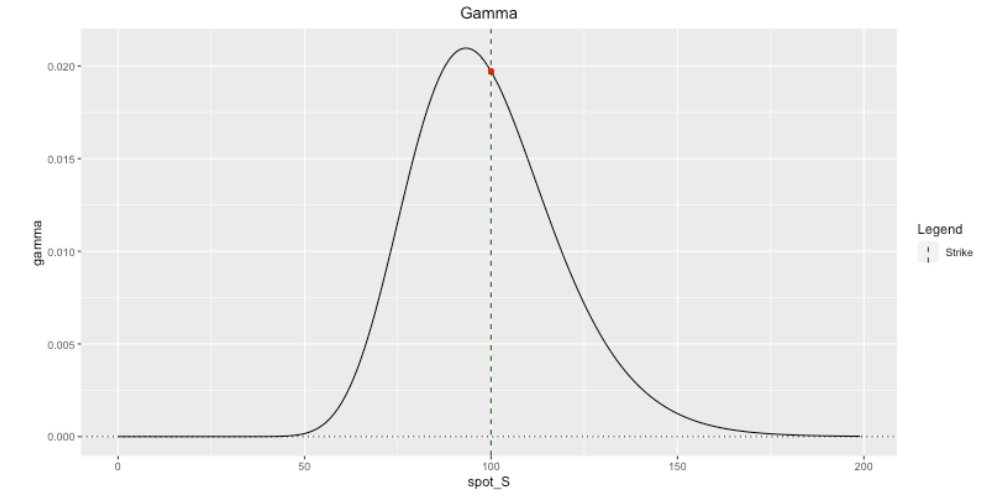
\includegraphics[scale=0.6]{gamma.png}
    \caption{Evolution du $\gamma$ en fonction du spot price $S$}
    \label{fig:enter-label}
\end{figure}

Par analogie, on peut comparer le delta à la vitesse et le gamma à l'accélération. Le gamma est une fonction décroissante de la maturité. 
Comme $\gamma_{call} \geq 0$ et $\gamma_{put} \geq 0$, on dit qu'un acheteur de call ou de put sera \textit{long de gamma}, ou que son portefeuille sera gamma positif, et qu'un vendeur sera court (short) de gamma, ou gamma négatif. Toutes choses égales par ailleurs, le gamma est maximum lorsque l'option est à la monnaie (i.e. lorsque $\delta_{option} = 0.5$). Un portefeuille comportant des positions acheteuses (dites longues) et vendeuses (dites courtes) d'options à différents prix d'exercice (sur un même sous-jacent) verra donc la valeur de son gamma évoluer, voire changer de signe, en fonction des évolutions du prix du sous-jacent. 
\subsubsection{Le thêta $\theta$}
Le thêta est le coût (ou le gain) du temps qui passe sur un portefeuille d'options. Il évalue combien le passage du temps influe sur la valeur d'une option. 
\begin{align*}
    \theta = - \frac{\partial P}{\partial t}
\end{align*}
En considérant des options européennes qui ne versent pas de dividendes
\begin{align*}
    \theta_{call} = -\frac{S N'(d_1) \sigma}{2 \sqrt{T}} - r K e^{- r T} N(d_2), \hspace{3mm} \theta_{put} = -\frac{S N'(d_1) \sigma}{2 \sqrt{T}} + r K e^{- r T} N(- d_2)
\end{align*}
\begin{figure}[H]
\subfloat[call tetha]{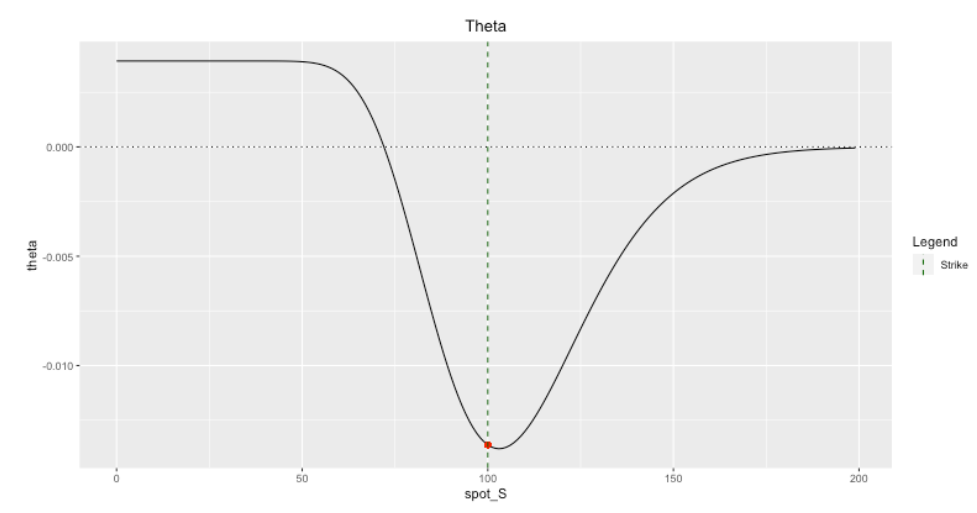
\includegraphics[scale=0.3]{theta.png}}
\subfloat[put theta]{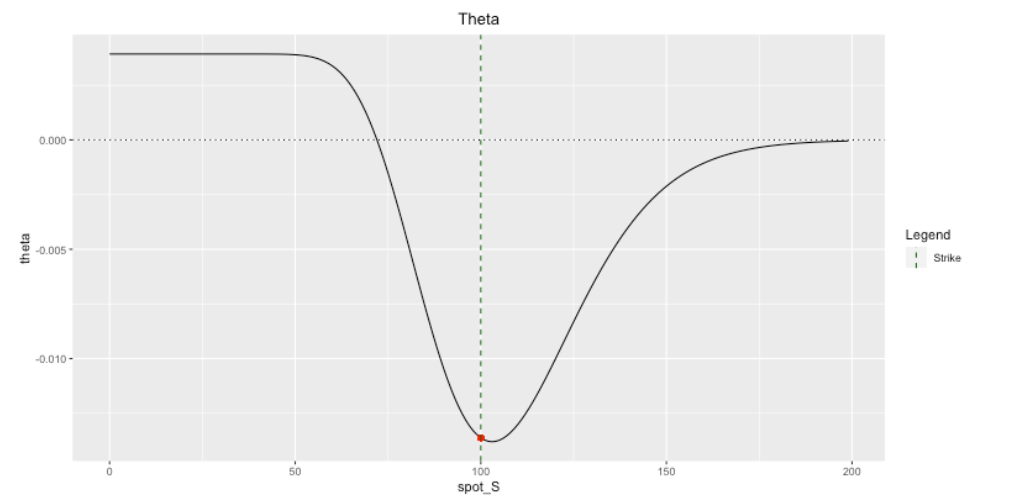
\includegraphics[scale=0.3]{put_theta.png}} \\
\caption{Evolution du $\theta$ de l'option}
\end{figure} 
Une position longue d'options (gamma positive) sera thêta négative. Le trader devra veiller tous les jours à payer son thêta journalier en profitant de sa position longue en gamma. On préfèrera donc être long d'une option qui soit suffisamment volatile, ainsi en rebalançant la position, on pourra payer le temps qui passe en tradant le gamma.
\subsubsection{Le rhô $\rho$}
Le rhô est le taux de variation de la valeur de la prime en fonction du taux sans risque.
\begin{align*}
    \rho = \frac{\partial P}{\partial r}, \hspace{2mm} \rho_{call} =  K T e^{- r T} N(d_2),  \hspace{2mm} \rho_{put} = - K T e^{- r T} N(- d_2)
\end{align*}

\begin{figure}[H]
\subfloat[call rho]{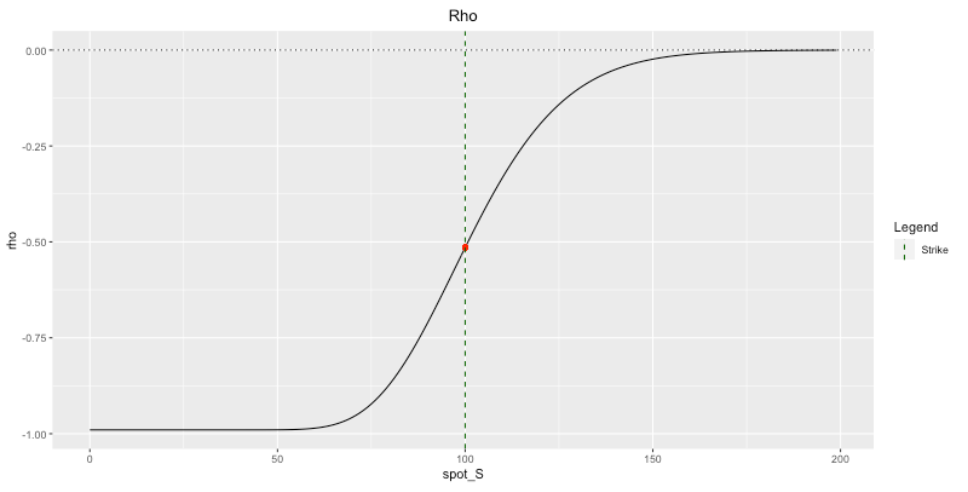
\includegraphics[scale=0.3]{put_rho.png}}
\subfloat[put rho]{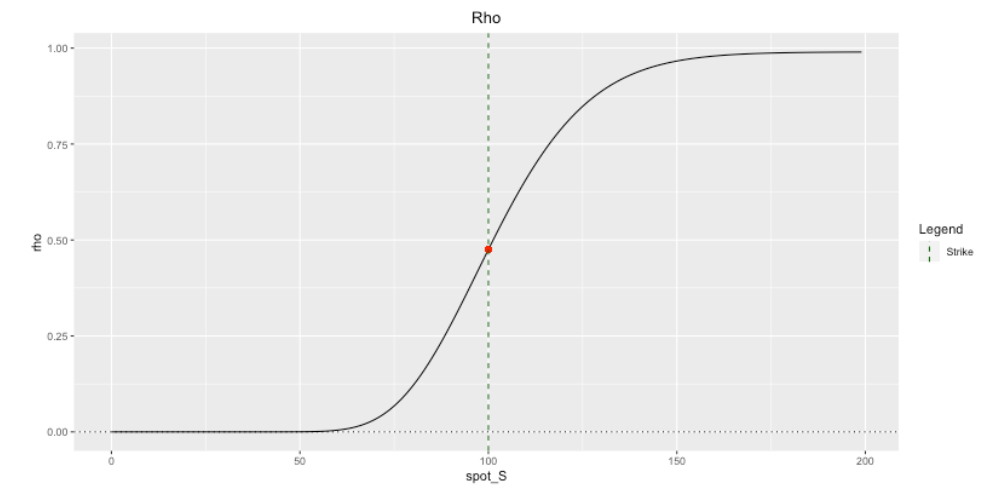
\includegraphics[scale=0.3]{call_rho.png}} 
\caption{Evolution du $\rho$ de l'option}
\end{figure} 

\subsubsection{le véga $\nu$}
Le véga mesure de la sensibilité à la volatilité implicite (voir modèle Black-Scholes)
\begin{align*}
    \nu_{call} = \nu_{put} = \frac{\partial P}{\partial \sigma} = S\sqrt{T} N'(d_1)
\end{align*}
Comme $\nu_{call}\geq 0$ et $\nu_{put}\geq 0$, on dit qu'un acheteur de call ou de put sera long de véga, ou que son portefeuille sera véga positif, et qu'un vendeur sera court (short) de véga, ou véga négatif. 

\subsubsection{Exemple d'utilisation}
an ATM call option price is \$7.97. The market parameters are the following:
\begin{itemize}
    \item underlying price \$100 (the stock does not pay any dividend)
    \item volatility 20\%
    \item rate of returns 0\%
    \item delta 54\%
    \item gamma 0.02
    \item vega 40
    \item theta -4
\end{itemize}
On peut alors poser les questions suivantes :
\begin{enumerate}[label=\textit{Q\arabic*.}]
    \item \textbf{Delta impact on price.} Quel sera le prix de l'option si celui du sous-jaçent augmente de \$1 ?
    \item \textbf{Gamma impact on Delta.} Si le gamma d'une option est de 0.04 et le delta est de 0.60, quel sera le nouveau delta si le prix sous-jacent augmente de \$1 ?
    \item \textbf{Vega Impact on Price.} Si la vega d'une option est de 30 et le prix de l'option est actuellement de \$5, combien le prix de l'option augmentera-t-il si la volatilité implicite augmente de 1\% ?
    \item \textbf{Theta Impact on Time.} Si l'option perd 0.05 de valeur par jour en raison du theta, combien de valeur perdra-t-elle en une semaine ?
    \item \textbf{Delta Hedging.} Vous détenez une position longue dans un call option avec un delta de 0.70 et un delta neutre à l'aide d'actions. Combien d'actions devrez-vous détenir pour neutraliser complètement la sensibilité au prix sous-jacent de l'option ?
    \item \textbf{Vega Hedging.} Si vous détenez une option avec une vega de 25 et vous souhaitez vous couvrir contre une augmentation de la volatilité implicite de 5 points de pourcentage, combien de contrats d'options devrez-vous acheter ou vendre pour vous couvrir ?
    \item \textbf{Theta Decay Analysis.} Vous détenez une position longue dans une option dont le theta est -0.03. Combien de valeur votre option perdra-t-elle au bout d'un mois en raison de la décroissance temporelle ?
    \item \textbf{Impact of Volatility on Price.} Vous détenez un call option avec un vega de 40. Si la volatilité implicite augmente de 2 points de pourcentage, de combien le prix de l'option augmentera-t-il ?
\end{enumerate}

\section{Options éxotiques}

\subsection{Options barrière}
On distingue plusieurs types d'options barrière, on peut les classer selon quatres groupes 
\begin{itemize}
    \item \textbf{Knock-In \& Up (UI):} Les options Up\&In naissent lorsque la barrière est touchée, sachant que le spot au départ du sous-jaçent se situe en dessous du niveau de barrière.
    \item \textbf{Knock-Out \& Up (UO):} Les options Up\&Out meurent lorsque la barrière est touchée, sachant que le spot au départ du sous-jaçent se situe en dessous du niveau de barrière.
    \item \textbf{Knock-In \& Down (DI):} Les options Down\&In naissent lorsque la barrière est touchée, sachant que le spot au départ du sous-jaçent se situe au dessus du niveau de barrière.
    \item \textbf{Knock-Out \& Down (DO):} Les options Down\&Out meurent lorsque la barrière est touchée, sachant que le spot au départ du sous-jaçent se situe au dessus du niveau de barrière.
\end{itemize}

\subsection{Baskets}
\subsubsection{Définition}
Les baskets sont des options barrière sur plusieurs sous-jaçents corrélés entre eux. On constate à chaque date d'observation la performance du basket. On considère plusieurs type de \textit{performances}:
\begin{itemize}
    \item \textbf{Worst-of/Best-of:} La performance du basket est donnée par l'actif présentant la pire (resp. meilleure) performance du basket.

    \item \textbf{Basket:} La performance est donné par la moyenne des performances de chaque actif, pondérée par le poids que représente  l'actif dans le basket.

    \item \textbf{Memory:} La performance est donnée par chaque actif relativement à sa barrière par rapport à son spot à la date d'observation. Le basket est rappelé si chaque actif a tapé sa barrière au moins une fois pendant la durée d'existence du basket. Il n'y a pas besoin que tous les actifs tapent en même temps leurs barrière, un effet de \textit{mémoire} est appliqué pendant toute la durée du basket.
\end{itemize}
\subsubsection{Matrice de corrélation}

\begin{definition}
    On considère un basket de sous-jaçents $S_1, S_2, \dots, S_n$ répartis selon des poids $w_1, w_2, \dots, w_n$. La realized correlation du basket est la quantité
    \begin{equation*}
        \rho_{r} = \frac{\sum_{1\leq i < j \leq n} w_{i}w_{j}\rho_{i,j}}{\sum_{1\leq i < j \leq n} w_{i}w_{j}}
    \end{equation*}
\end{definition}

\begin{theorem}
    La relation entre la variance du basket et la corrélation est
    \begin{equation}
        \sigma_{ptf}² = \sum_{i=1}^n w_{i}^2\sigma_i^2+ 2\sum_{1\leq i < j \leq n} w_{i}w_{j}\sigma_i \sigma_j \rho_{i,j}
    \end{equation}
\end{theorem}

\subsubsection{Corrélation implicite}

On considère deux options: une option (européenne) sur un index (par exmple sur le S\&P500) et un basket option sur l'ensemble des actifs composants l'indice. On peut alors introduire une corrélation implicite dérivée de la volatilité réelle donné par le marché.

\begin{definition}
    La corrélation implicite de l'index est une mesure de la dépendance entre un indice et ses composants
    \begin{equation*}
        \rho_{index\text{ }implied} = \frac{\sigma_{index}^2 - \sum_{i=1}^n w_{i}^2\sigma_i^2 }{2\sum_{1\leq i < j \leq n} w_{i}w_{j}\sigma_i \sigma_j \rho_{i,j}}
    \end{equation*}
\end{definition}

\subsection{Autocallables}

\subsubsection{Description}

Les autocalls (automatically callable) sont des produits structurés qui ont la particularité de pouvoir être rappelé en cas de dépassement de barrière (AB) à des dates d'observation définies à l'émission. Ils donne aussi la possibilité à l'investisseur de recevoir des coupons à des dates d'observation si la barrière Coupon (CB) n'est pas tapée. Les barrières Coupon et Autocall (CB et AB) peuvent être les mêmes ou être différentes. Le pay-off d'un autocall contient deux composantes, le Coupon et le Rachat:
\begin{equation*}
    Coupon(t_i) = N * C\% * \mathbb{1}\{
\end{equation*}

\subsection{Hedge d'une option barrière}

Pour hedger une option barrière, le trader va acheter un \textit{call spread}.

\section{Etude de cas -- Stochastic repo hybrid model}

\subsection{Repo rate dynamics}

\subsection{Linear Gaussian Markov model (LGM)}

\subsection{Exchanges rate model}

\subsection{Pricing dans une devise étrangère}

\subsection{Calibration des corrélations}

\subsubsection{Quanto options}
\subsubsection{Hybrid stock/funding exchange}
\subsubsection{Hybrid basket}

\section{Dérivés de Crédit}

\section{Modèles de regression}
 \subsection{Décomposition biais--variance}
 Le cadre général des modèles statistiques est le suivant. On suppose que les données $x_i$ sont liés aux variables $y_i$ par la relation
 \begin{equation}
     y_i = f(x_i) + \epsilon_i
 \end{equation}
 Où $f$ est une fonction inconnue et $\epsilon_i$  suit une loi normale de moyenne nulle et de variance $\sigma^2$. Le but de la regression est de trouver une fonction $\hat{f}$ qui approxime le mieux $f$ en tenant le moins possible compte de $\epsilon_i$. Ainsi, on cherche à minimiser l'erreur au carré moyenne qui peut etre décomposée sous la forme
 \begin{equation}
     \mathbb{E}\bigg[(y-\hat{f}(x))^2\bigg] = \underbrace{\mathbb{E}\bigg[f(x_i)-\hat{f}(x) \bigg]^2}_{\text{biais}} +
     \underbrace{\mathbb{E}\bigg[f(x_i)^2\bigg]-\mathbb{E}\bigg[\hat{f}(x)\bigg]^2}_{\text{variance}} +
     \sigma^2
 \end{equation}
 On peut interpréter les différents termes comme
 \begin{itemize}
     \item Le biais $\mathbb{E}[f(x_i)-\hat{f}(x) ]^2$ représente à quel point le modèle $\hat{f}$ approxime la fonction $f$
     \item la variance \[ \mathbb{E}[f(x_i)^2]-\mathbb{E}[\hat{f}(x)]^2\]représente le niveau de variabilité de $\hat{f}$ sans tenir compte de $f$
     \item $\sigma^2$ représente le niveau de bruit de $(y_i, x_i)$
 \end{itemize}

 Les méthodes de régression sont largement utilisées en finance de marché pour modéliser et analyser les relations entre différentes variables. Ces méthodes permettent aux professionnels de la finance d'analyser les données historiques, de prévoir les tendances futures, de mesurer les risques et de prendre des décisions éclairées.
 \subsection{Moindres carrés (OLS)}
 \textbf{Cadre théorique.} On considère un échantillon $(Y_i, X_{i_1}, \dots , X_{i_n})$. On cherche à estimer la \textit{variable endogène}  $Y_i$ à partir des \textit{variables explicatives} $(X_{i_1}, \dots , X_{i_n})$
 \begin{equation}
     Y_i = a_{i1}X_{i1} + \dots + a_{in}X_{in} + \epsilon_i
 \end{equation}
 Ce qui donne sous forme matricielle, avec $\textbf{Y}$ de dimension $(n,1)$, $\textbf{X}$ de dimension $(n,p+1)$, $a$ de dimension $(p+1,1)$, $\epsilon$ de dimension $(n,1)$, $n$ le nombre d'observations et $p$ le nombre de variables explicatives,
 \begin{equation}
     \textbf{Y} = \textbf{X} a + \epsilon
 \end{equation}
On va estimer les paramètres $(a_i)_{0\leq i \leq p+1}$ afin d'obtenir
\begin{align*}
    \hat{y_i} = \hat{a_0} + \hat{a_1}x_{i,1} + \dots + \hat{a_p}x_{i,p}
\end{align*}
La méthode des moindres carrés consiste à minimiser la somme des carrés des résidus, à savoir
\begin{equation}
    \min \sum_{i=1}^{n} \hat{\epsilon_i^2} = \min_{\hat{a_0}, \dots, \hat{a_p}} \sum_{i=1}^{n} (\hat{y_i} - \hat{a_0} - \hat{a_1}x_{i,1} - \dots - \hat{a_p}x_{i,p})^2
\end{equation}
\textbf{Théorème.} La solution de ce problème est
\begin{equation}
    \hat{a} = (\textbf{X}^T \textbf{X})^{-1} \textbf{X}^T \textbf{Y}
\end{equation}
C'est un estimateur sans biai i.e. $\mathbb{E}[\hat{a}]=a$.

\subsection{Regression Ridge ($L^2$)}
On rappelle le système linéaire de notre modèle. 
\[
\begin{bmatrix}
y_1 \\
y_2 \\
\vdots \\
y_n \\
\end{bmatrix} = 
\begin{bmatrix}
1 & x_1^{(1)} & x_1^{(2)} & \cdots & x_1^{(q)} \\
1 & x_2^{(1)} & x_2^{(2)} & \cdots & x_2^{(q)} \\
\vdots & \vdots & \ddots & \vdots \\
1 & x_n^{(1)} & x_n^{(2)} & \cdots & x_n^{(q)} \\
\end{bmatrix}
\begin{bmatrix}
\beta_0 \\
\beta_1 \\
\vdots \\
\beta_q \\
\end{bmatrix}
+
\begin{bmatrix}
\epsilon_0 \\
\epsilon_1 \\
\vdots \\
\epsilon_n \\
\end{bmatrix}
\]
L regression ridge impose une contrainte $L^2$ sur les coefficients pour éviter qu'ils partent dans tous les sens. On cherche donc à trouver
\begin{align}
    \min_{\beta_1, \dots, \beta_p} \sum_{i=1}^{n} \bigg( y_i - \sum_{k=1}^{p} \beta_k z_{i,k} \bigg)^2
\end{align}
Sous la contrainte 
\begin{align*}
    \sum_{i=1}^{n} \beta_i ^2 \leq \tau
\end{align*}
Avec $\tau$ un paramètre à fixer. Les variables de base $X_i$ on été centrées réduites en $Z_i$ pour éviter que les variables à trop haute variance n'aient trop d'influence.
\\
\vspace{1mm}
\\
On peut montrer que le problème est équivalent à ajouter une \textit{pénalité} à la fonction à minimiser. On cherche alors un paramètre $\lambda \geq 0$ et on cherche
\begin{align}
    \hat{\beta} =\underset{{\beta \in \mathbb{R}^p}}{\operatorname{argmin}}  ||Y-X\beta||^2 + \lambda ||\beta||^2 
\end{align}
\textbf{Théorème.} L'estimateur ridge s'écrit alors:
\begin{equation}
    \hat{\beta} = (\textbf{X}^T \textbf{X} +\lambda\textbf{I}_p )^{-1} \textbf{X}^T \textbf{Y}
\end{equation}
\textit{Démonstration.} \begin{proof} Posons notre fonction de coùt qu'on cherche à minimiser
\begin{equation}
    J_{\lambda}(\beta) = ||Y-X\beta||^2 + \lambda ||\beta||^2 = (Y-X\beta)^T(Y-X\beta) + \lambda \beta^T \beta
\end{equation}
En développant on obtient 
\begin{equation*}
    J_{\lambda}(\beta) = Y^T Y - 2X^T Y + \beta^T (X^T X + \lambda I_p) \beta 
\end{equation*}
Comme la matrice $X^T X + \lambda I_p$ est symétrique on utilise la propriété
\begin{equation}
    \frac{\partial x^T A x}{\partial x} = 2 A x \text{  , pour $A$ symétrique.}
\end{equation}
On obtient alors l'estimateur $\hat{\beta}$ tel que
\begin{equation*}
    \partial_{\beta} J_{\lambda} (\hat{\beta}) = 0 \Leftrightarrow (X^T X + \lambda I_p) \hat{\beta} = X^T Y
\end{equation*}
Et on obtient le résultat.\\
\textbf{Note.} Avec un raisonnement similaire on peut obtenir l'estimateur MCO (LSE) et on pourra introduire la matrice pseudo inverse de $X$
\begin{equation}
    X^{\dagger} = (X^T X)^{-1}X^T 
\end{equation}
\end{proof}
\begin{figure}[H]
    \centering
    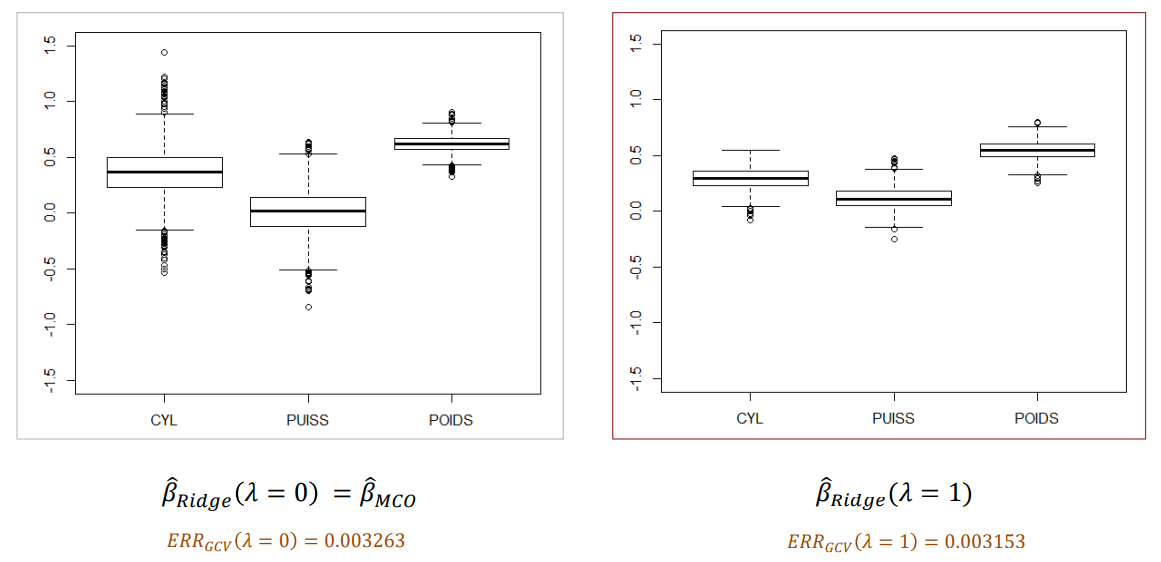
\includegraphics[scale=0.5]{ridge_perfo.png}
    \caption{Stabilisation des coefficients avec Ridge}
    \label{fig:enter-label}
\end{figure}
C’est un petit exemple $(n = 27, p = 3)$, le gap de performances n’est pas très flamboyant. En revanche, la réduction de la variance des coefficients estimés saute aux yeux.
\\
On peut déterminer la valeur de $\lambda$ de manière empirique ou par le calcul. On trouve alors les estimateur LSO et on a deux calcul \textit{Hoerl, Kennard, Baldwin (1975)} et \textit{Lawless, Wang (1976)}
\begin{equation*}
    \lambda_{HKB} = \frac{(p-2)\hat{\sigma_\epsilon}^2}{\sum \hat{\beta_j} ^2} \text{  et  } \lambda_{LW} = \frac{n(p-2)\hat{\sigma_\epsilon}^2}{\sum \hat{y_j} ^2}
\end{equation*}
\subsection{Regression Lasso ($L^1$)}
\subsubsection{Enoncé du problème}
Tout comme la regression Ridge, on impose ici une pénalité mais cette fois-ci de type $L^1$ sur les coéfficients c'est-à-dire
\begin{align}
    \min_{\beta_1, \dots, \beta_p} \sum_{i=1}^{n} \bigg( y_i - \sum_{k=1}^{p} \beta_k z_{i,k} \bigg)^2
\end{align}
Sous la contrainte 
\begin{align*}
    \sum_{i=1}^{n} |\beta_i| \leq \tau
\end{align*}
Qu'on peut écrire de manière équivalente
\begin{align}
    \min_{\beta_1, \dots, \beta_p} \sum_{i=1}^{n} \bigg( y_i - \sum_{k=1}^{n} \beta_k z_{i,k} \bigg)^2 + \lambda \sum_{i=1}^{p} |\beta_i| 
\end{align}
\textbf{Quel intérêt par rapport à Ridge ?} La regression Lasso peut faire office de dispositif de
sélection de variables en annulant certains coefficients $\beta_j$: les variables associées
à $(\beta_j = 0)$ sont de facto exclues du modèle prédictif.
\subsubsection{Forward Stagewise Algorithm}
Il n’y a pas de calcul direct pour la regression Lasso. On résoud alors par un algorithme (LARS ou FSA). C’est une démarche itérative où l’on commence avec tous les $(\beta_j = 0)$. On fait évoluer les coefficients sélectivement

\begin{figure}[H]
    \centering
    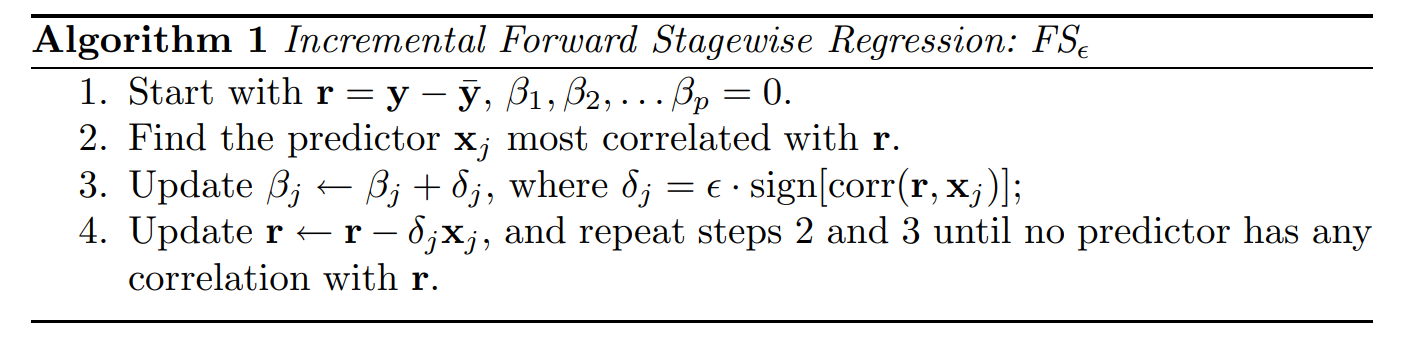
\includegraphics[scale=0.4]{algo.png}
    \caption{Forward Stagewise Algorithm}
    \label{fig:enter-label}
\end{figure}

Dans l’optique prédictive, la minimisation de l’erreur de prédiction en balayant les valeurs de $\lambda$
reste la méthode la plus efficace. On procède souvent par validation croisée

\begin{figure}[H]
    \centering
    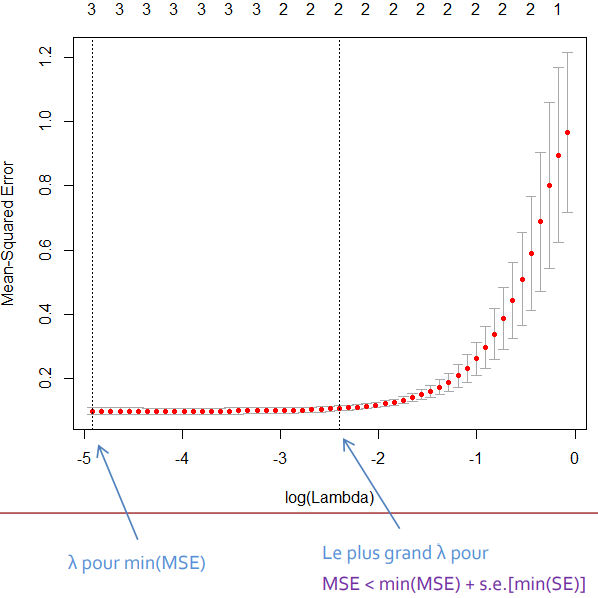
\includegraphics[scale=0.7]{lasso.png}
    \caption{Choix du paramètre $\lambda$}
    \label{fig:enter-label}
\end{figure}

En résumé:
\begin{itemize}
    \item \textbf{(+)} Capacité à sélectionner les variables en acceptant les coefficients nuls
    \item \textbf{(--)} Dans les problèmes à très grandes dimensions $(p >> n)$, LASSO ne sélectionne que $n$ variables prédictives au maximum, mécaniquement. C’est une vraie limitation de l’algorithme.
    \item \textbf{(--)} Parmi un groupe de variables corrélées, LASSO en choisit une, \textbf{celle qui est la plus liée à a cible souvent}, masquant l’influence des autres. Cet inconvénient est inhérent aux techniques intégrant un mécanisme de sélection de variables
\end{itemize}


\section{Méthodes numériques}

 \subsection{Monte Carlo}

\subsubsection{Algorithme de base}
\subsubsection{Réduction de variance}
\subsubsection{Markov Chain Monte Carlo}
 
 \subsection{Résolutions de PDE}

 \subsubsection{Adjoint Algorithmic Differentiation}
  \texttt{https://quant.opengamma.io/Adjoint-Algorithmic-Differentiation-OpenGamma.pdf}
  \\
  \vspace{0.5mm}
  \\
 L'adjoint algorithmique de différentiation est une technique utilisée pour calculer les gradients de fonctions numériques efficacement et précisément. Il est souvent utilisé en finance pour le calcul des sensibilités (ou des "Greeks") de produits financiers complexes tels que les options et les dérivés.\\
 L'idée principale de l'adjoint algorithmique de différentiation est de calculer les gradients en résolvant un système d'équations différentielles, appelé équations adjointes, qui est dérivé du calcul original. Ce système d'équations adjointes peut être résolu de manière très efficace par rapport aux techniques de différenciation numérique classiques telles que la différence finie.
\\
En utilisant l'adjoint algorithmique de différentiation, il est possible de calculer les \textbf{sensibilités des portefeuilles de produits financiers complexes de manière plus rapide et plus précise, ce qui peut être crucial pour les stratégies de trading et de gestion des risques.}


\subsubsection{Finite Differences}
Les différences finies sont une méthode numérique utilisée en finance pour calculer les prix et les sensibilités de produits financiers tels que les options, les futures et les obligations. La méthode des différences finies consiste à discrétiser les équations différentielles qui sous-tendent les modèles financiers continus, en les transformant en une série d'équations discrètes qui peuvent être résolues numériquement.
\\
En utilisant les différences finies, les traders et les gestionnaires de risques peuvent calculer les prix et les sensibilités de produits financiers complexes de manière efficace et précise, en fonction des paramètres tels que la volatilité du marché, les taux d'intérêt et les dividendes. 
\begin{lstlisting}[language=Python]
S, K, T, r, sigma = 100, 105, 1, 0.05, 0.2 

# Inputs pour le maillage
N, M = 100, 100 # Nombre de pas de temps et d'espace
dt = T/N # Pas de temps
dx = np.sqrt(dt)*sigma # Pas d'espace
x_max = 5*sigma*np.sqrt(T) # Valeur maximale de x
x_min = -x_max # Valeur minimale de x
x_values = np.linspace(x_min, x_max, M+1)

# Initialisation des tableaux
u_old = np.zeros(M+1)
u_new = np.zeros(M+1)

# Conditions aux limites
u_old[0] = 0
u_old[M] = np.maximum(S - K*np.exp(x_max), 0)

# Calcul de u_new
for i in range(1, N+1):
    # Conditions aux limites pour chaque pas de temps
    u_new[0] = 0
    u_new[M] = np.maximum(S - K*np.exp(x_max), 0)
    
    # Boucle de calcul pour chaque point d'espace
    for j in range(1, M):
        a = 0.5*sigma**2*(x_values[j]**2) - r*x_values[j]
        b = -sigma**2*(x_values[j]**2) - r
        c = 0.5*sigma**2*(x_values[j]**2) + r*x_values[j]
        u_new[j] = (a*u_old[j-1] + b*u_old[j] + c*u_old[j+1])/(1+r*dt)
    
    # Mise a jour de u_old pour le prochain pas de temps
    u_old = u_new.copy()

# Calcul du prix de l'option
price = np.interp(np.log(S/K), x_values, u_new)
\end{lstlisting}

\section{Neural Networks}

\subsection{Artificial Neural Network}
\subsubsection{Motivations}
Les régressions linéaires assument une relation linéaire entre les variables indépendantes et dépendantes. Cependant, de nombreuses relations dans les données réelles peuvent être non linéaires. Les réseaux de neurones, avec leurs fonctions d'activation non linéaires, sont capables de capturer des relations complexes et flexibles entre les entrées et les sorties.
\\
\vspace{0.5mm}
\\
\textbf{Exemple. XOR} On cherche ici à modéliser la porte XOR (non-linéaire). On dispose alors d'un dataset d'entrée
\begin{align*}
    \mathcal{D} = \bigg\{ ((0,0)^T, 0), ((1,0)^T, 1), ((0,1)^T, 1), ((1,1)^T, 0) \bigg\}
\end{align*}
En utilisant une regression de type LSE, on cerche alors à minimiser la foncion cout
\begin{align*}
    J(\beta) = ||Y-W^T X - w_0||^2
\end{align*}
Et on a la fonction estimée $Y(X)= W^T X + w_0$. Cependant, à cause de la non-linéarité, on trouve comme solution optimale $W=0$ et $w_0=0.5$ i.e. $Y(X)=0.5$ partout.
\\
\vspace{1mm}
\\
On choisit alors de construire un 2-layer perceptron:
\begin{figure}[H]
    \centering
    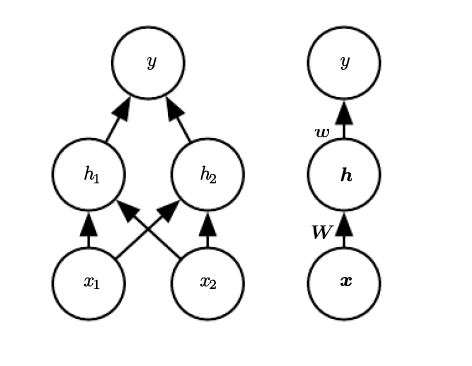
\includegraphics[scale=0.7]{2-layer.png}
    \caption{Two-layer perceptron}
    \label{fig:enter-label}
\end{figure}
Les caractéristiques sont les suivantes:
\begin{itemize}
    \item \textbf{Hidden unit.} $h= g(W^T x + c)$ Avec $g(\alpha) = \max (0,\alpha)$
    \item \textbf{Sortie.} La sortie est $y=w^T h + b$ Soit $y= w^T\max (0, W^T x + c) + b$
    \item \textbf{Loss function.} La fonction de perte à minimiser est l'erreur LSE
    \begin{align*}
        J(\beta) = \frac{1}{N} \sum_{n=1}^{N} (t_n - y(x_n))^2
    \end{align*}
\end{itemize}
La solution optimale est alors 
\begin{align*}
    W= \text{mat}(1,1,1,1), c=(0, -1)^T, w=(1,-2)^T, b=0
\end{align*}
\subsubsection{Fonctionnement}


Un réseau de neurones artificiels (\textit{Artificial Neural Network, Multilayer Perceptron, Feedforward Neural Network}) est un modèle informatique qui est inspiré par le fonctionnement du cerveau humain. Il est composé de plusieurs unités appelées neurones, organisées en couches, et ces neurones sont connectés les uns aux autres. Il se compose de plusieurs caractéristiques clés:
\begin{itemize}
    \item \textbf{Entrées :} Le processus commence avec la couche d'entrée, qui représente \textbf{les données d'entrée du modèle}. Chaque neurone dans cette couche correspond à une caractéristique ou à une dimension des données d'entrée. Par exemple, dans le cas de la reconnaissance d'image, chaque neurone de la couche d'entrée pourrait représenter \textbf{la valeur d'un pixel.}

    \item \textbf{Poids et biais :} Chaque connexion entre les neurones de deux couches consécutives est associée à un \textbf{poids}. Les poids sont des paramètres ajustables qui modifient l'influence d'une entrée sur la sortie d'un neurone. \textbf{Un biais} est également ajouté à chaque neurone pour introduire un certain niveau de flexibilité dans le modèle.

    \item \textbf{Somme pondérée :} Pour chaque neurone dans la couche suivante (\textit{hiddel layer}), la somme pondérée des entrées (multipliées par les poids correspondants) est calculée, et le biais est ajouté. \textbf{Cette somme pondérée est ensuite passée à travers une fonction d'activation.}

    \item \textbf{Fonction d'activation :} La fonction d'activation introduit de la non-linéarité dans le modèle. Elle détermine si et dans quelle mesure un neurone doit être activé. Différentes fonctions d'activation, telles que la sigmoïde, la tangente hyperbolique, ou la ReLU (Rectified Linear Unit), peuvent être utilisées.

    \item \textbf{Propagation avant :} Ce processus de calcul de la somme pondérée, d'ajout du biais, d'application de la fonction d'activation \textbf{est répété pour chaque couche} jusqu'à ce que les sorties soient générées par la couche de sortie. C'est ce qu'on appelle la propagation avant (\textit{forward propagation}).

    \item \textbf{Fonction de perte :} Les sorties du réseau sont comparées aux valeurs attendues à l'aide d'une fonction de perte (\textit{loss function}). La fonction de perte mesure l'écart entre les prédictions du réseau et les valeurs réelles. L'objectif lors de l'entraînement du réseau est de minimiser cette fonction de perte.

    \item \textbf{Rétropropagation :} Pour ajuster les poids et les biais afin de minimiser la fonction de perte, on utilise un algorithme d'optimisation. La rétropropagation du gradient (\textit{backpropagation}) est l'algorithme le plus couramment utilisé. Il calcule les gradients de la fonction de perte par rapport aux poids du réseau, puis ajuste les poids en conséquence pour réduire l'erreur.

    \item \textbf{Apprentissage :} La propagation avant, suivi de la rétropropagation, est répété sur plusieurs itérations (époques) jusqu'à ce que le réseau apprenne à effectuer la tâche souhaitée de manière satisfaisante. Les poids et les biais sont ajustés itérativement pendant cette phase d'apprentissage.
\end{itemize}

\begin{figure}[H]
    \centering
    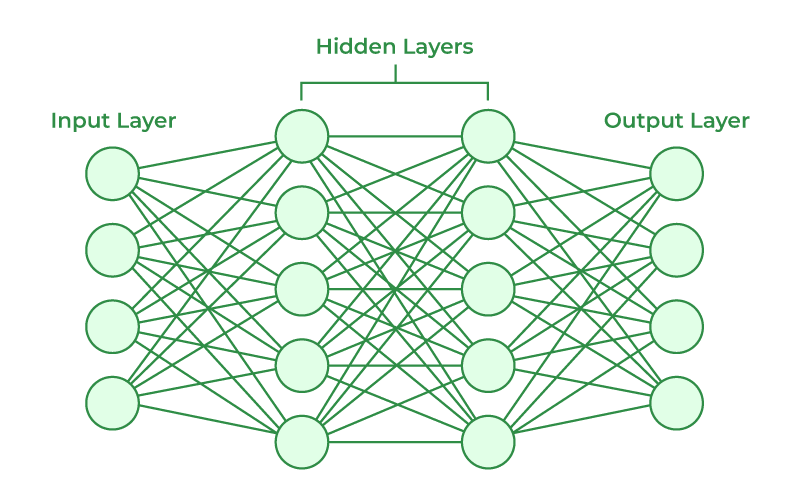
\includegraphics[scale=0.4]{ann.png}
    \caption{Artificial Neural Network}
    \label{fig:enter-label}
\end{figure}

\subsubsection{Ouput units}

On considère la sortie d'un \textit{hidden layer} $h= f(x, \theta^{n-1})$. On cherche alors la sortie $y= f(h, \theta^{n})$ ainsi que la fonction de perte $J(\theta)$. On trouve alors 
\begin{itemize}
    \item Regression
    \item Binary classification
    \item Multi-class classification
\end{itemize}

\subsubsection{Fonctions d'activation}
La fonction d'activation est une fonction appliquée à un signal en sortie d'un neurone artificiel. Le terme de "fonction d'activation" vient de l'équivalent biologique "potentiel d'activation", seuil de stimulation qui, une fois atteint entraîne une réponse du neurone.
\\
\vspace{2mm}
\\
\textbf{Propriétés. } On utilise souvent des fonctions qui ont les propriétés suivantes:
\begin{enumerate}[label=\textit{(\roman*)}]
    \item \textbf{Non-linéarité.} permet au réseau de neurones de modéliser des relations complexes et non linéaires entre les variables d'entrée et de sortie.
    \item \textbf{Différentiabilité.} Partout différentiable, cela facilite l'optimisation du réseau à l'aide de techniques telles que la rétropropagation du gradient.
    \item \textbf{Etendue.} Quand l'étendue est finie, les méthodes d'apprentissage basées sur les gradients sont plus stables (impact sur un nombre de poids limités). Quand l'étendue est infinie, l'apprentissage est généralement plus efficace (impact sur davantage de poids).
    \item \textbf{Monotonie de la dérivée} Les fonctions à dérivée monotone ont été montrées comme ayant une meilleure capacité à généraliser dans certains cas. \ding{79}
\end{enumerate} 

\textbf{Exemples de fonctions d'activation} 

\begin{table}[H]
    \centering
    \begin{tabular}{|c|c|c|c|c|}
        \hline
        Nom & Graphe & Expression & Dérivée & Étendue \\
        \hline
        Heaviside & 
        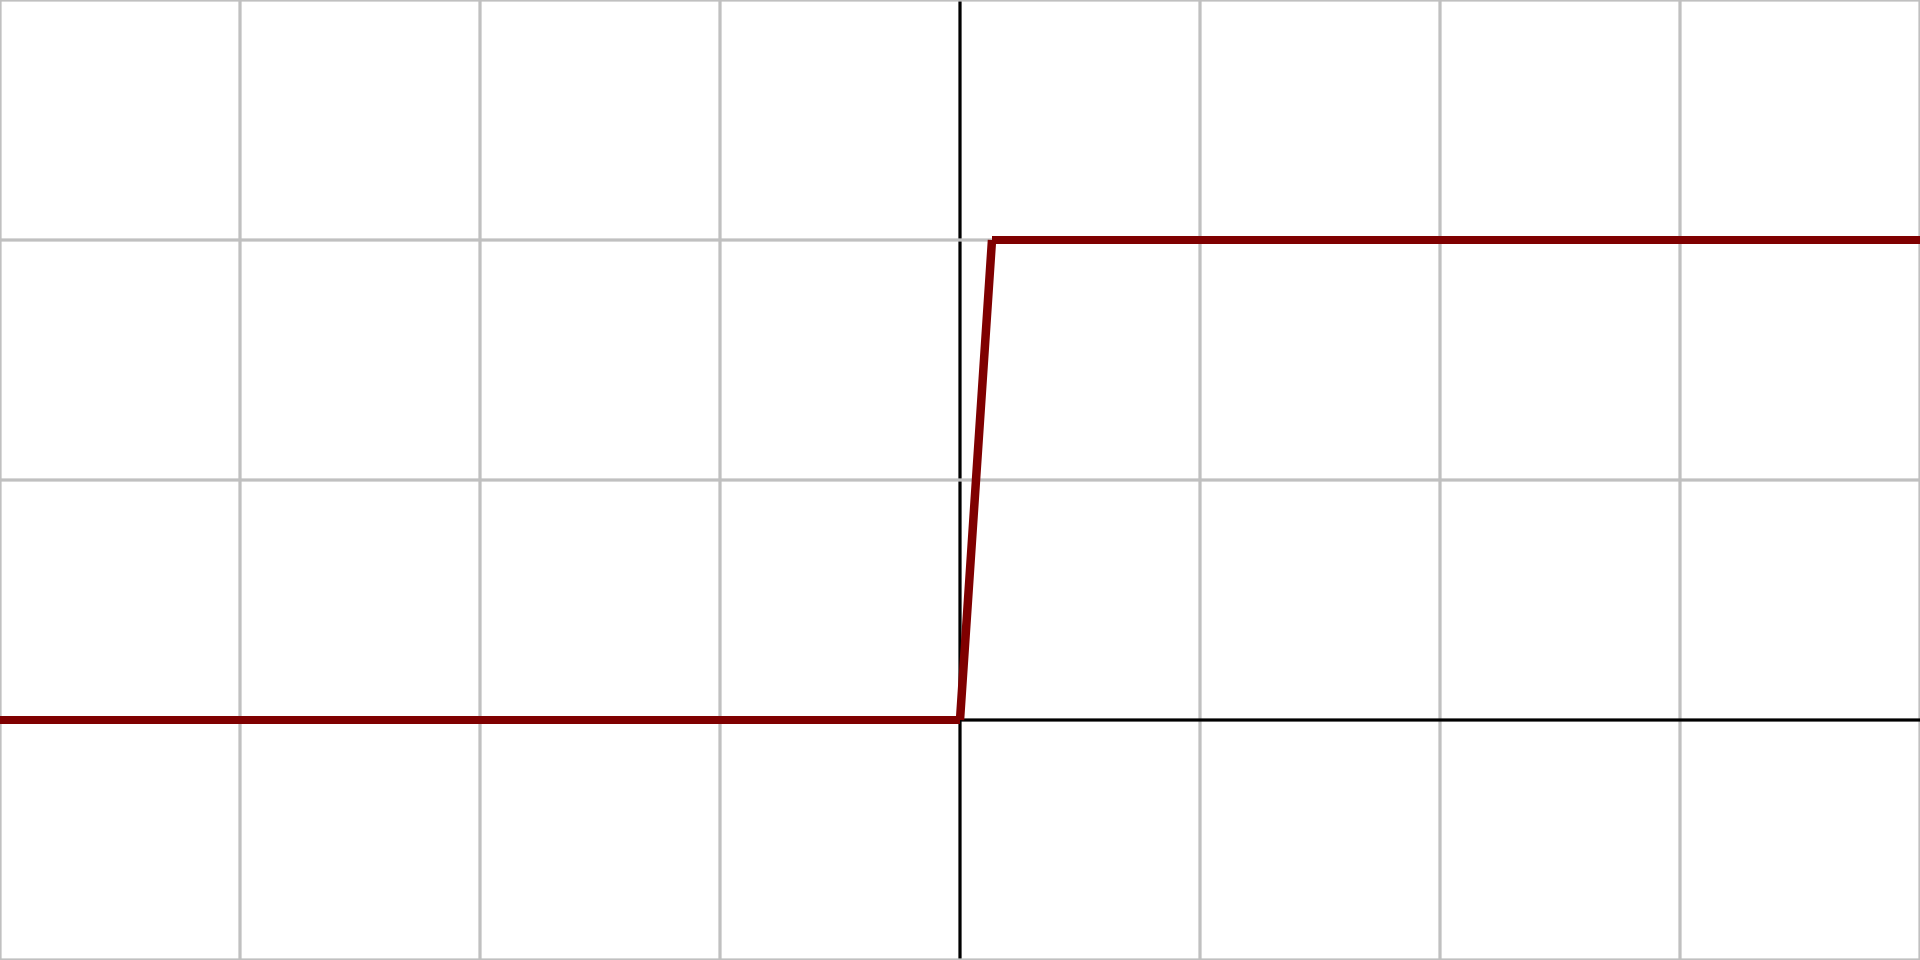
\includegraphics[width=1.5cm]{heavyside_graph.png} & 
        $H(x) = \begin{cases} 0, & \text{si } x < 0 \\ 1, & \text{si } x \geq 0 \end{cases}$ & 
        $\delta(x)$ & 
        $\{0, 1\}$ \\
        \hline
        Sigmoïde & 
        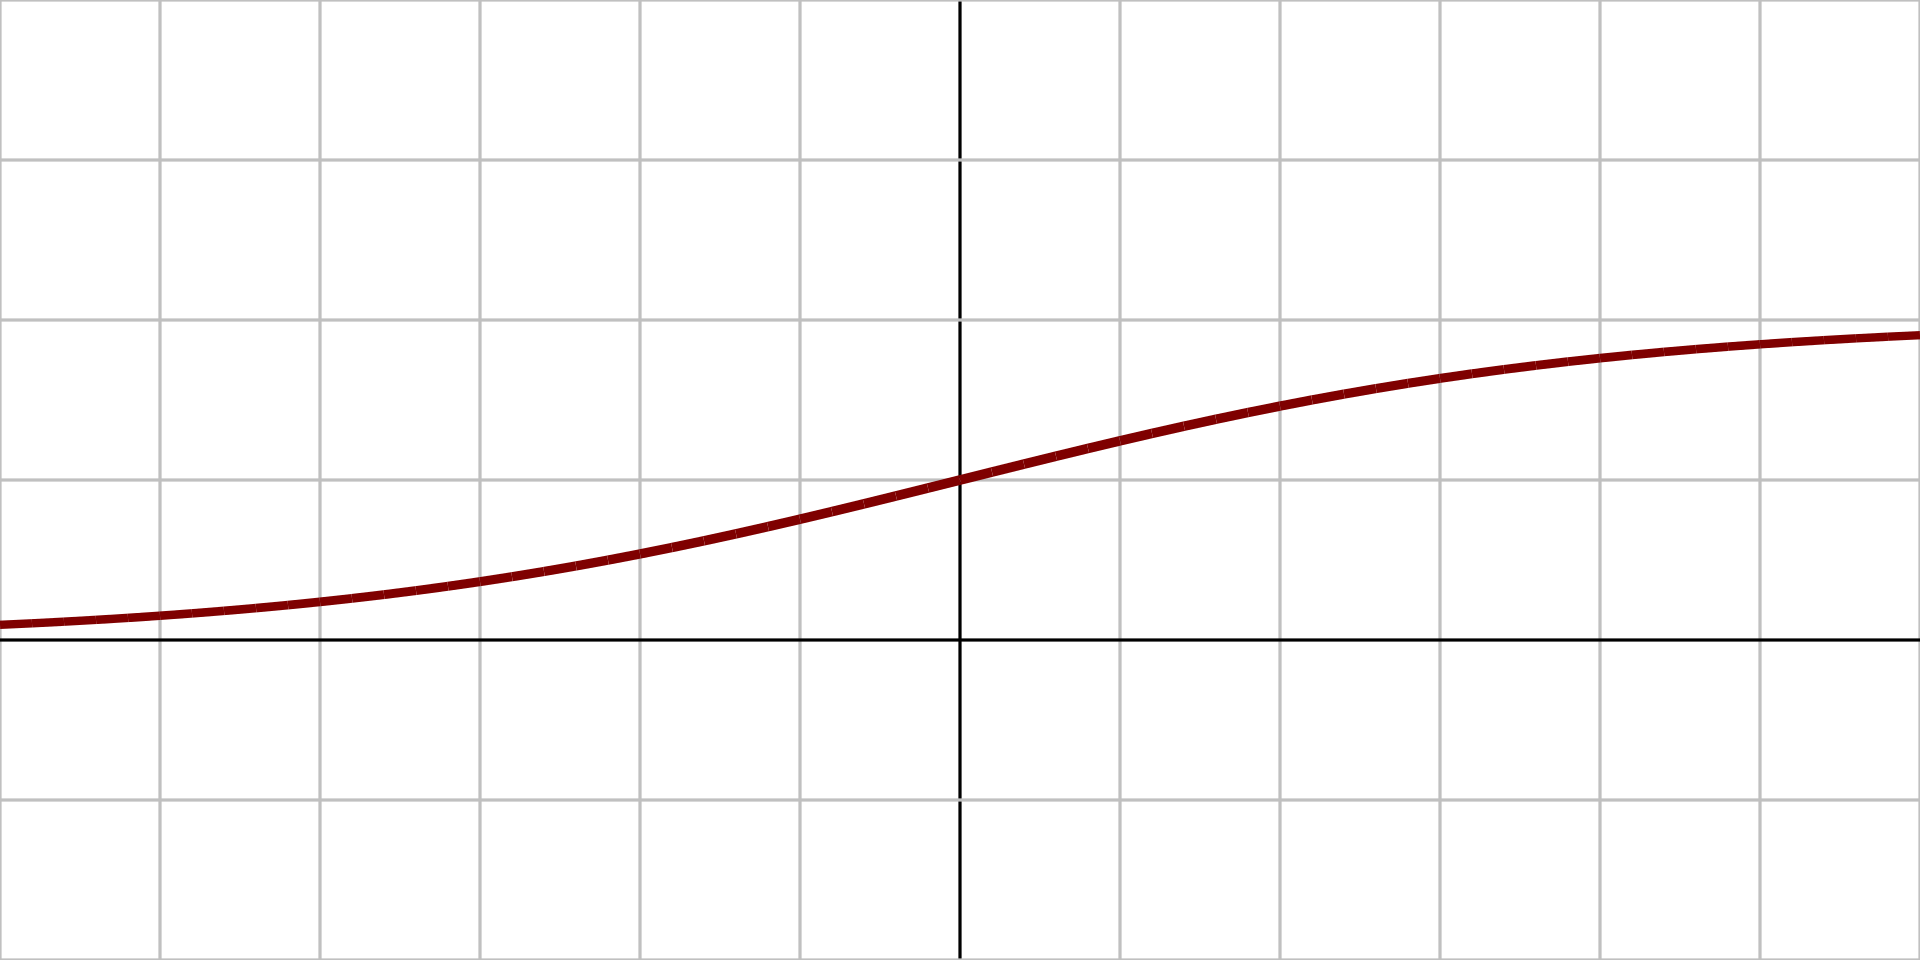
\includegraphics[width=1.5cm]{sigmoid_graph.png} & 
        $\sigma(x) = \frac{1}{1 + e^{-x}}$ & 
        $\sigma'(x) = \sigma(x)(1 - \sigma(x))$ & 
        $[0, 1]$ \\ 
        \hline
        ReLU & 
        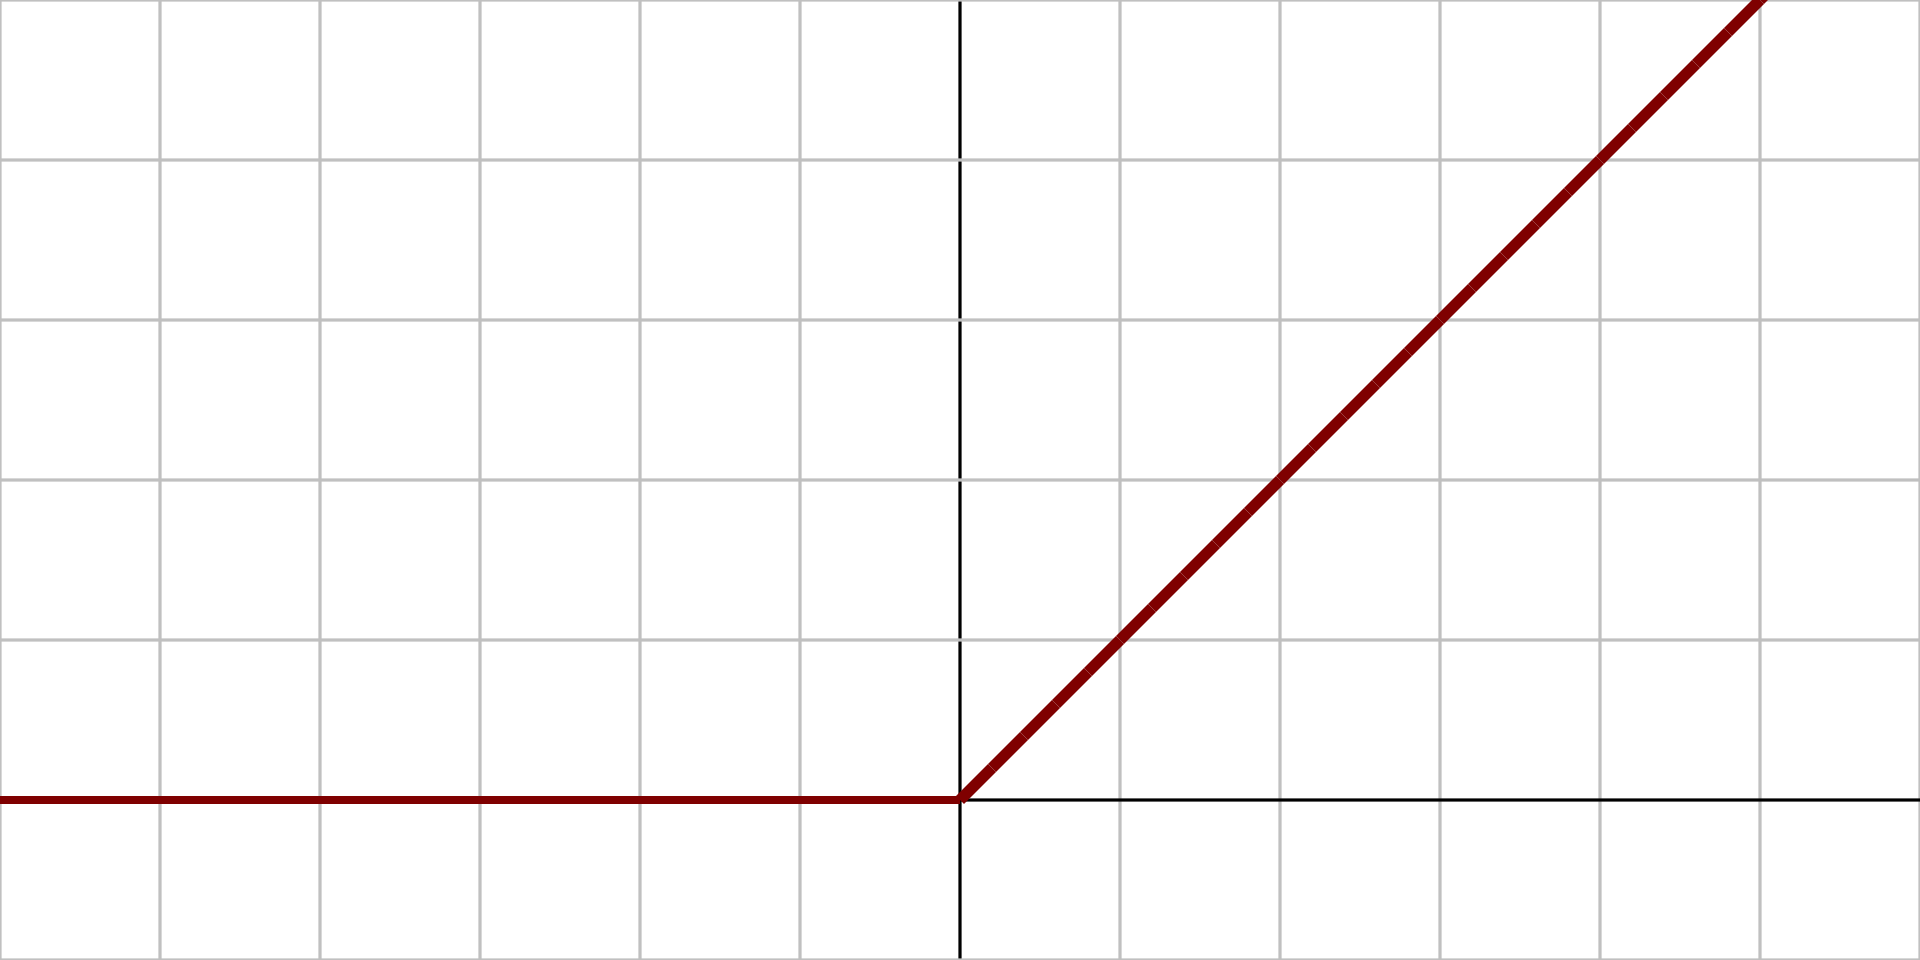
\includegraphics[width=1.5cm]{relu_graph.png} & 
        $\text{ReLU}(x) = \max(0, x)$ & 
        $\text{ReLU}'(x) = \begin{cases} 0, & \text{si } x < 0 \\ 1, & \text{si } x \geq 0 \end{cases}$ & 
        $\mathbb{R}$ \\ 
        \hline
        Tanh & 
        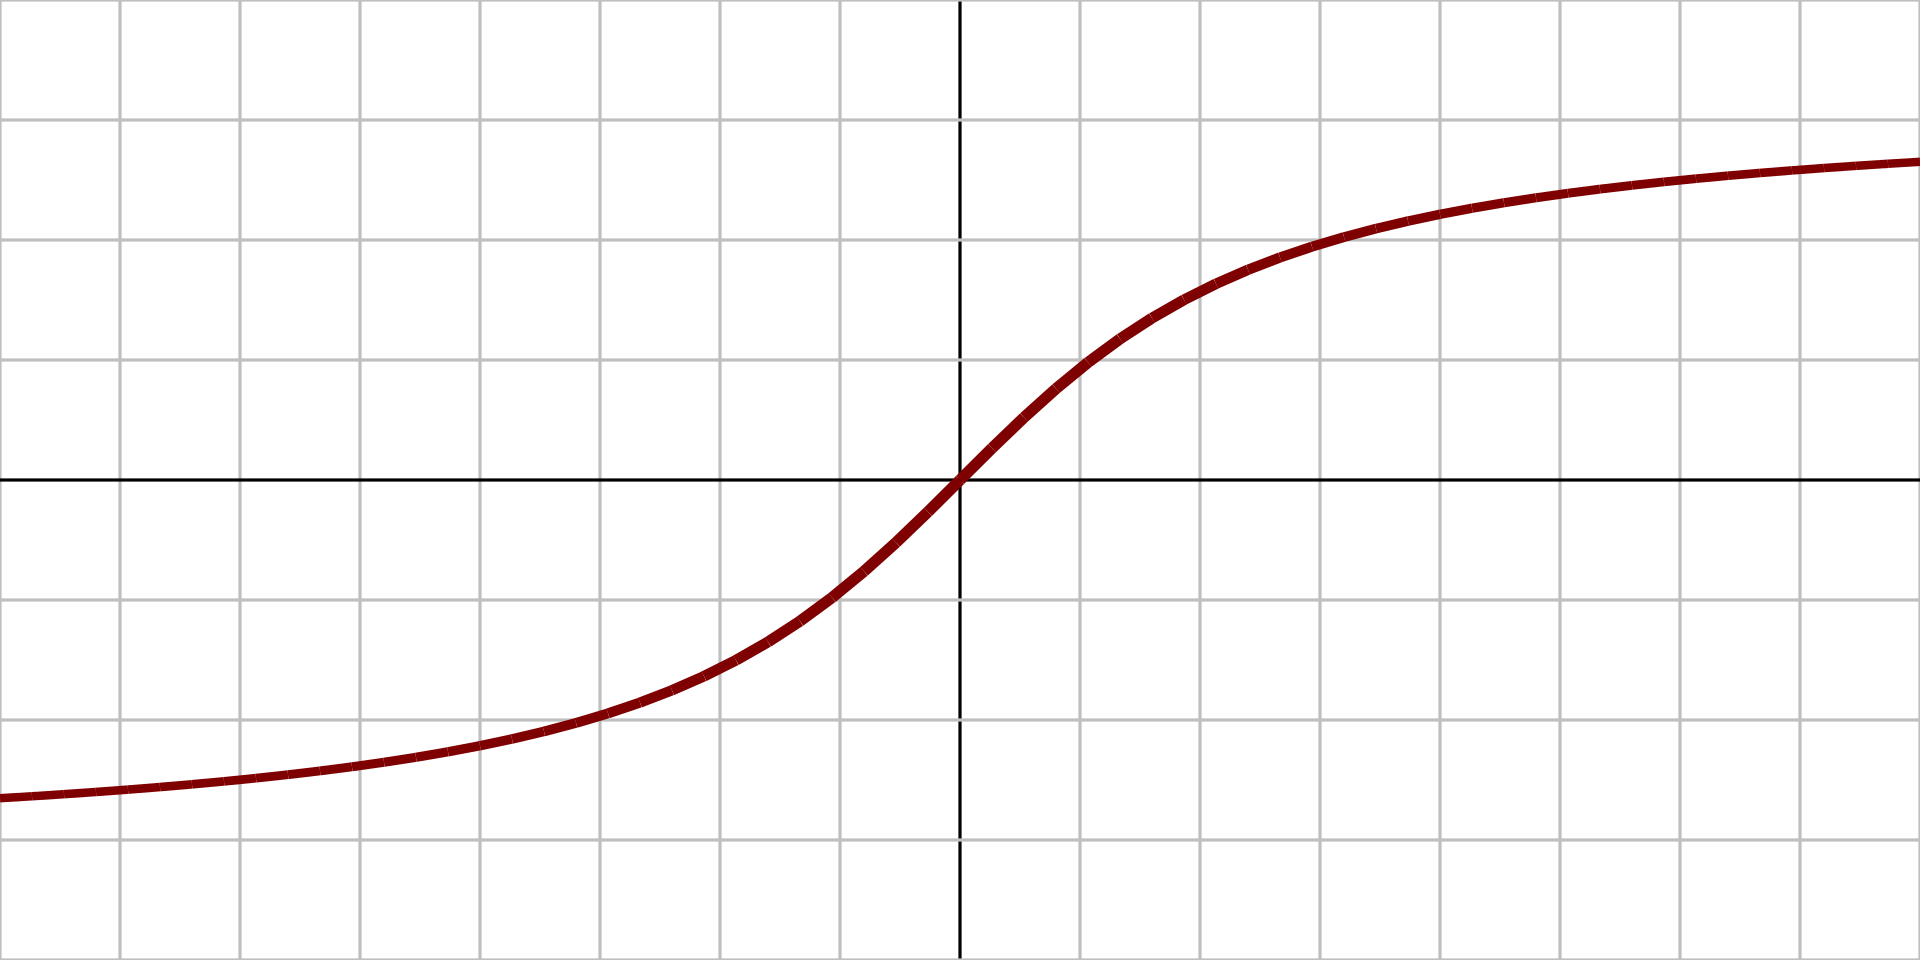
\includegraphics[width=1.5cm]{arctangent_graph.png} & 
        $\tanh(x) = \frac{e^{2x} - 1}{e^{2x} + 1}$ & 
        $\tanh'(x) = 1 - \tanh^2(x)$ & 
        $[-1, 1]$ \\ \\
        \hline
    \end{tabular}
    \caption{Tableau des fonctions d'activation}
    \label{tab:activation_functions}
\end{table}

\section{Brainteasers}

\end{document}